% Options for packages loaded elsewhere
\PassOptionsToPackage{unicode}{hyperref}
\PassOptionsToPackage{hyphens}{url}
%
\documentclass[
]{article}
\usepackage{amsmath,amssymb,verbatim}
\usepackage{lmodern}
\usepackage{ifxetex,ifluatex}
\ifnum 0\ifxetex 1\fi\ifluatex 1\fi=0 % if pdftex
  \usepackage[T1]{fontenc}
  \usepackage[utf8]{inputenc}
  \usepackage{textcomp} % provide euro and other symbols
\else % if luatex or xetex
  \usepackage{unicode-math}
  \defaultfontfeatures{Scale=MatchLowercase}
  \defaultfontfeatures[\rmfamily]{Ligatures=TeX,Scale=1}
\fi
% Use upquote if available, for straight quotes in verbatim environments
\IfFileExists{upquote.sty}{\usepackage{upquote}}{}
\IfFileExists{microtype.sty}{% use microtype if available
  \usepackage[]{microtype}
  \UseMicrotypeSet[protrusion]{basicmath} % disable protrusion for tt fonts
}{}
\makeatletter
\@ifundefined{KOMAClassName}{% if non-KOMA class
  \IfFileExists{parskip.sty}{%
    \usepackage{parskip}
  }{% else
    \setlength{\parindent}{0pt}
    \setlength{\parskip}{6pt plus 2pt minus 1pt}}
}{% if KOMA class
  \KOMAoptions{parskip=half}}
\makeatother
\usepackage{xcolor}
\IfFileExists{xurl.sty}{\usepackage{xurl}}{} % add URL line breaks if available
\IfFileExists{bookmark.sty}{\usepackage{bookmark}}{\usepackage{hyperref}}
\hypersetup{
  pdftitle={Statistical Learning Project},
  pdfauthor={Filippo Santin, Gurjeet Singh, Francesca Zen},
  hidelinks,
  pdfcreator={LaTeX via pandoc}}
\urlstyle{same} % disable monospaced font for URLs
\usepackage[margin=1in]{geometry}
\usepackage{color}
\usepackage{fancyvrb}
\newcommand{\VerbBar}{|}
\newcommand{\VERB}{\Verb[commandchars=\\\{\}]}
\DefineVerbatimEnvironment{Highlighting}{Verbatim}{commandchars=\\\{\}}
% Add ',fontsize=\small' for more characters per line
\usepackage{framed}
\definecolor{shadecolor}{RGB}{248,248,248}
\newenvironment{Shaded}{\begin{snugshade}}{\end{snugshade}}
\newcommand{\AlertTok}[1]{\textcolor[rgb]{0.94,0.16,0.16}{#1}}
\newcommand{\AnnotationTok}[1]{\textcolor[rgb]{0.56,0.35,0.01}{\textbf{\textit{#1}}}}
\newcommand{\AttributeTok}[1]{\textcolor[rgb]{0.77,0.63,0.00}{#1}}
\newcommand{\BaseNTok}[1]{\textcolor[rgb]{0.00,0.00,0.81}{#1}}
\newcommand{\BuiltInTok}[1]{#1}
\newcommand{\CharTok}[1]{\textcolor[rgb]{0.31,0.60,0.02}{#1}}
\newcommand{\CommentTok}[1]{\textcolor[rgb]{0.56,0.35,0.01}{\textit{#1}}}
\newcommand{\CommentVarTok}[1]{\textcolor[rgb]{0.56,0.35,0.01}{\textbf{\textit{#1}}}}
\newcommand{\ConstantTok}[1]{\textcolor[rgb]{0.00,0.00,0.00}{#1}}
\newcommand{\ControlFlowTok}[1]{\textcolor[rgb]{0.13,0.29,0.53}{\textbf{#1}}}
\newcommand{\DataTypeTok}[1]{\textcolor[rgb]{0.13,0.29,0.53}{#1}}
\newcommand{\DecValTok}[1]{\textcolor[rgb]{0.00,0.00,0.81}{#1}}
\newcommand{\DocumentationTok}[1]{\textcolor[rgb]{0.56,0.35,0.01}{\textbf{\textit{#1}}}}
\newcommand{\ErrorTok}[1]{\textcolor[rgb]{0.64,0.00,0.00}{\textbf{#1}}}
\newcommand{\ExtensionTok}[1]{#1}
\newcommand{\FloatTok}[1]{\textcolor[rgb]{0.00,0.00,0.81}{#1}}
\newcommand{\FunctionTok}[1]{\textcolor[rgb]{0.00,0.00,0.00}{#1}}
\newcommand{\ImportTok}[1]{#1}
\newcommand{\InformationTok}[1]{\textcolor[rgb]{0.56,0.35,0.01}{\textbf{\textit{#1}}}}
\newcommand{\KeywordTok}[1]{\textcolor[rgb]{0.13,0.29,0.53}{\textbf{#1}}}
\newcommand{\NormalTok}[1]{#1}
\newcommand{\OperatorTok}[1]{\textcolor[rgb]{0.81,0.36,0.00}{\textbf{#1}}}
\newcommand{\OtherTok}[1]{\textcolor[rgb]{0.56,0.35,0.01}{#1}}
\newcommand{\PreprocessorTok}[1]{\textcolor[rgb]{0.56,0.35,0.01}{\textit{#1}}}
\newcommand{\RegionMarkerTok}[1]{#1}
\newcommand{\SpecialCharTok}[1]{\textcolor[rgb]{0.00,0.00,0.00}{#1}}
\newcommand{\SpecialStringTok}[1]{\textcolor[rgb]{0.31,0.60,0.02}{#1}}
\newcommand{\StringTok}[1]{\textcolor[rgb]{0.31,0.60,0.02}{#1}}
\newcommand{\VariableTok}[1]{\textcolor[rgb]{0.00,0.00,0.00}{#1}}
\newcommand{\VerbatimStringTok}[1]{\textcolor[rgb]{0.31,0.60,0.02}{#1}}
\newcommand{\WarningTok}[1]{\textcolor[rgb]{0.56,0.35,0.01}{\textbf{\textit{#1}}}}
\usepackage{longtable,booktabs,array}
\usepackage{calc} % for calculating minipage widths
% Correct order of tables after \paragraph or \subparagraph
\usepackage{etoolbox}
\makeatletter
\patchcmd\longtable{\par}{\if@noskipsec\mbox{}\fi\par}{}{}
\makeatother
% Allow footnotes in longtable head/foot
\IfFileExists{footnotehyper.sty}{\usepackage{footnotehyper}}{\usepackage{footnote}}
\makesavenoteenv{longtable}
\usepackage{graphicx}
\makeatletter
\def\maxwidth{\ifdim\Gin@nat@width>\linewidth\linewidth\else\Gin@nat@width\fi}
\def\maxheight{\ifdim\Gin@nat@height>\textheight\textheight\else\Gin@nat@height\fi}
\makeatother
% Scale images if necessary, so that they will not overflow the page
% margins by default, and it is still possible to overwrite the defaults
% using explicit options in \includegraphics[width, height, ...]{}
\setkeys{Gin}{width=\maxwidth,height=\maxheight,keepaspectratio}
% Set default figure placement to htbp
\makeatletter
\def\fps@figure{htbp}
\makeatother
\setlength{\emergencystretch}{3em} % prevent overfull lines
\providecommand{\tightlist}{%
  \setlength{\itemsep}{0pt}\setlength{\parskip}{0pt}}
\setcounter{secnumdepth}{-\maxdimen} % remove section numbering
\ifluatex
  \usepackage{selnolig}  % disable illegal ligatures
\fi

\title{Statistical Learning Project\\ \textit{EDA for stroke clinical cases}}
\author{Filippo Santin \qquad \qquad Gurjeet Singh \qquad \qquad Francesca Zen\\
2020627\quad \qquad \qquad \qquad 2004251 \qquad \qquad \quad \qquad 2010640}
\date{22/6/2021}

\begin{document}
\maketitle

\hypertarget{introduction}{%
\section{1 Introduction}\label{introduction}}

In the following report, we present a study computed on stroke
disease in which we try to explain from statistical analysis some
correlation factors and statistics of the given features, by designing
models to predict the presence of stroke disease. In addition, we will
highlight possible linear and non-linear relationships among the given
features (predictors) and the stroke disease variable (predicted
variable).

``Stroke'' is the medical term for damage to brain tissue or the death
of a portion of it, due to insufficient blood supply to an area of the
brain. According to the World Health Organization (WHO) stroke is the
2nd leading cause of death globally, responsible for approximately 11\%
of total deaths and our aim is to see if and how the variables we are
dealing with are related to each other, in order to predict which individual is more probable to have a stroke.\\
The symptoms of stroke vary from patient to patient, depending on the
severity of the condition, the affected brain area, causes, type of
stroke, etc. Stroke is characterized by sudden onset and for this reason
it involves the need for immediate therapeutic intervention and adapted
to the needs of the patient. In this sense, looking for relation between
features may help to prevent or assess it.

In order to have a guide for the interpretation of the data, we underline
the following information:

\begin{itemize}
\tightlist
\item
  The normal values of glucose level are between 60 and 110 mg/dl and
  with a value greater than 126 mg/dl a person is considered diabetic;
\item
  a body mass index (BMI) between 18.5-24.9 indicates a normal/healthy
  weight, below 18.5 indicates underweight, 25.0-29.9 indicates
  overweight and above 30.0 indicates obese person.
\end{itemize}

\hypertarget{exploring-the-dataset}{%
\section{2 Exploring the Dataset}\label{exploring-the-dataset}}

The dataset we used is provided by Kaggle \footnote{\url{https://www.kaggle.com/fedesoriano/stroke-prediction-dataset}}
and it is composed of 5,110 entries with a total of 12 columns:
\texttt{id}, \texttt{gender}, \texttt{age}, \texttt{hypertension},
\texttt{heart\_disease}, \texttt{ever\_married}, \texttt{work\_type},
\texttt{Residence\_type}, \texttt{avg\_glucose\_level}, \texttt{bmi},
\texttt{smoking\_status}, \texttt{stroke}.

\begin{Shaded}
\begin{Highlighting}[]
\FunctionTok{library}\NormalTok{(knitr)}
\NormalTok{stroke\_data }\OtherTok{\textless{}{-}} \FunctionTok{read.csv}\NormalTok{(}\StringTok{\textquotesingle{}healthcare{-}dataset{-}stroke{-}data.csv\textquotesingle{}}\NormalTok{)}
\FunctionTok{kable}\NormalTok{(stroke\_data[}\DecValTok{1}\SpecialCharTok{:}\DecValTok{5}\NormalTok{,], }\AttributeTok{format =} \StringTok{\textquotesingle{}simple\textquotesingle{}}\NormalTok{, }\AttributeTok{align=}\StringTok{\textquotesingle{}ccccccccc\textquotesingle{}}\NormalTok{, }
      \AttributeTok{col.names =} \FunctionTok{c}\NormalTok{(}\StringTok{\textquotesingle{}id\textquotesingle{}}\NormalTok{,}\StringTok{\textquotesingle{}gender\textquotesingle{}}\NormalTok{,}\StringTok{\textquotesingle{}age\textquotesingle{}}\NormalTok{, }\StringTok{\textquotesingle{}hypert.\textquotesingle{}}\NormalTok{, }\StringTok{\textquotesingle{}hd\textquotesingle{}}\NormalTok{ ,}\StringTok{\textquotesingle{}ev\_marr\textquotesingle{}}\NormalTok{,}
                    \StringTok{\textquotesingle{}work\_type\textquotesingle{}}\NormalTok{,}\StringTok{\textquotesingle{}res\_type\textquotesingle{}}\NormalTok{,}\StringTok{\textquotesingle{}glucose\textquotesingle{}}\NormalTok{, }\StringTok{\textquotesingle{}bmi\textquotesingle{}}\NormalTok{,}\StringTok{\textquotesingle{}smoking\textquotesingle{}}\NormalTok{,}\StringTok{\textquotesingle{}stroke\textquotesingle{}}\NormalTok{))}
\end{Highlighting}
\end{Shaded}
\newpage
\setlength\LTleft{-1cm}
\begin{longtable}[]{@{}cccccccccccc@{}}
\toprule
id & gender & age & hypert. & hd & ev\_marr & work\_type & res\_type &
glucose & bmi & smoking & stroke \\
\midrule
\endhead
9046 & Male & 67 & 0 & 1 & Yes & Private & Urban & 228.69 & 36.6 &
formerly smoked & 1 \\
51676 & Female & 61 & 0 & 0 & Yes & Self-employed & Rural & 202.21 & N/A
& never smoked & 1 \\
31112 & Male & 80 & 0 & 1 & Yes & Private & Rural & 105.92 & 32.5 &
never smoked & 1 \\
60182 & Female & 49 & 0 & 0 & Yes & Private & Urban & 171.23 & 34.4 &
smokes & 1 \\
1665 & Female & 79 & 1 & 0 & Yes & Self-employed & Rural & 174.12 & 24 &
never smoked & 1 \\
\bottomrule
\caption{Few samples of the dataset}\label{samples_of_dataset}
\end{longtable}

In Table \ref{samples_of_dataset} we can see an overview of the characteristics of people in the dataset.

\hypertarget{preprocessing}{%
\subsection{2.1 Preprocessing}\label{preprocessing}}

The preliminary part of the analysis focuses on the study of the dataset
and its pre-processing: we looked at the \texttt{id} column and verified
that all the data collected refer to different people, thus no
recidivist status was involved.\\
After this check we removed the column from the dataset since it does not
hold useful information for our study.

\begin{Shaded}
\begin{Highlighting}[]
\NormalTok{stroke\_data }\OtherTok{\textless{}{-}}\NormalTok{ stroke\_data[,}\SpecialCharTok{{-}}\DecValTok{1}\NormalTok{]}
\end{Highlighting}
\end{Shaded}

In order to use the variables through the analysis we transformed the
categorical variables into factors:

\begin{Shaded}
\begin{Highlighting}[]
\NormalTok{stroke\_data}\SpecialCharTok{$}\NormalTok{gender }\OtherTok{\textless{}{-}} \FunctionTok{as.factor}\NormalTok{(stroke\_data}\SpecialCharTok{$}\NormalTok{gender)}
\NormalTok{stroke\_data}\SpecialCharTok{$}\NormalTok{ever\_married }\OtherTok{\textless{}{-}} \FunctionTok{as.factor}\NormalTok{(stroke\_data}\SpecialCharTok{$}\NormalTok{ever\_married)}
\NormalTok{stroke\_data}\SpecialCharTok{$}\NormalTok{work\_type }\OtherTok{\textless{}{-}} \FunctionTok{as.factor}\NormalTok{(stroke\_data}\SpecialCharTok{$}\NormalTok{work\_type)}
\NormalTok{stroke\_data}\SpecialCharTok{$}\NormalTok{Residence\_type }\OtherTok{\textless{}{-}} \FunctionTok{as.factor}\NormalTok{(stroke\_data}\SpecialCharTok{$}\NormalTok{Residence\_type)}
\NormalTok{stroke\_data}\SpecialCharTok{$}\NormalTok{smoking\_status }\OtherTok{\textless{}{-}} \FunctionTok{as.factor}\NormalTok{(stroke\_data}\SpecialCharTok{$}\NormalTok{smoking\_status)}
\NormalTok{stroke\_data}\SpecialCharTok{$}\NormalTok{heart\_disease}\OtherTok{\textless{}{-}}\FunctionTok{as.factor}\NormalTok{(stroke\_data}\SpecialCharTok{$}\NormalTok{heart\_disease)}
\end{Highlighting}
\end{Shaded}

The variable \texttt{bmi} was not numeric because of the presence of
``N/A'' string values which identify missing information, hence we
transformed its elements into numerical values and then removed the NA
values generated.

\begin{Shaded}
\begin{Highlighting}[]
\NormalTok{stroke\_data}\SpecialCharTok{$}\NormalTok{bmi }\OtherTok{\textless{}{-}} \FunctionTok{as.numeric}\NormalTok{(stroke\_data}\SpecialCharTok{$}\NormalTok{bmi)}
\end{Highlighting}
\end{Shaded}

\begin{verbatim}
## Warning: NAs introduced by coercion
\end{verbatim}

\begin{Shaded}
\begin{Highlighting}[]
\NormalTok{stroke\_data }\OtherTok{\textless{}{-}} \FunctionTok{na.omit}\NormalTok{(stroke\_data)}
\end{Highlighting}
\end{Shaded}

We ended up having 4,909 entries and 11 total columns.\\
Here we give a quick overview of the main information about the dataset:

\begin{Shaded}
\begin{Highlighting}[]
\FunctionTok{summary}\NormalTok{(stroke\_data)}
\end{Highlighting}
\end{Shaded}

\begin{verbatim}
##     gender          age         hypertension    
##  Female:2897   Min.   : 0.08   Min.   :0.00000  
##  Male  :2011   1st Qu.:25.00   1st Qu.:0.00000  
##  Other :   1   Median :44.00   Median :0.00000  
##                Mean   :42.87   Mean   :0.09187  
##                3rd Qu.:60.00   3rd Qu.:0.00000  
##                Max.   :82.00   Max.   :1.00000  
##  heart_disease ever_married         work_type   
##  0:4666        No :1705     children     : 671  
##  1: 243        Yes:3204     Govt_job     : 630  
##                             Never_worked :  22  
##                             Private      :2811  
##                             Self-employed: 775  
##                                                 
##  Residence_type avg_glucose_level      bmi       
##  Rural:2419     Min.   : 55.12    Min.   :10.30  
##  Urban:2490     1st Qu.: 77.07    1st Qu.:23.50  
##                 Median : 91.68    Median :28.10  
##                 Mean   :105.31    Mean   :28.89  
##                 3rd Qu.:113.57    3rd Qu.:33.10  
##                 Max.   :271.74    Max.   :97.60  
##          smoking_status     stroke       
##  formerly smoked: 837   Min.   :0.00000  
##  never smoked   :1852   1st Qu.:0.00000  
##  smokes         : 737   Median :0.00000  
##  Unknown        :1483   Mean   :0.04257  
##                         3rd Qu.:0.00000  
##                         Max.   :1.00000
\end{verbatim}

\hypertarget{descriptive-statistic}{%
\subsection{2.2 Descriptive Statistic}\label{descriptive-statistic}}

\begin{Shaded}
\begin{Highlighting}[]
\FunctionTok{attach}\NormalTok{(stroke\_data)}
\end{Highlighting}
\end{Shaded}

In order to highlight and analize better the data, we use some plots to
study their statistics and distribution.\\
A relevant and important information is provided by the following
barplot, in which we highlight the unbalance dataset issue: \(209\) people on a
total of \(4909\) get a stroke, i.e.~the \(4.26 \%\) of the people.

\begin{Shaded}
\begin{Highlighting}[]
\FunctionTok{table}\NormalTok{(stroke)}
\end{Highlighting}
\end{Shaded}

\begin{verbatim}
## stroke
##    0    1 
## 4700  209
\end{verbatim}

\begin{Shaded}
\begin{Highlighting}[]
\FunctionTok{table}\NormalTok{(stroke)}\SpecialCharTok{/}\FunctionTok{dim}\NormalTok{(stroke\_data)[}\DecValTok{1}\NormalTok{]}
\end{Highlighting}
\end{Shaded}

\begin{verbatim}
## stroke
##          0          1 
## 0.95742514 0.04257486
\end{verbatim}

\begin{Shaded}
\begin{Highlighting}[]
\FunctionTok{barplot}\NormalTok{(}\FunctionTok{table}\NormalTok{(stroke)}\SpecialCharTok{/}\FunctionTok{dim}\NormalTok{(stroke\_data)[}\DecValTok{1}\NormalTok{], }\AttributeTok{xlab=}\StringTok{\textquotesingle{}stroke\textquotesingle{}}\NormalTok{,}
        \AttributeTok{col =} \FunctionTok{c}\NormalTok{(}\StringTok{\textquotesingle{}\#F8766D\textquotesingle{}}\NormalTok{,}\StringTok{\textquotesingle{}\#00BFC4\textquotesingle{}}\NormalTok{))}
\end{Highlighting}
\end{Shaded}

\begin{center}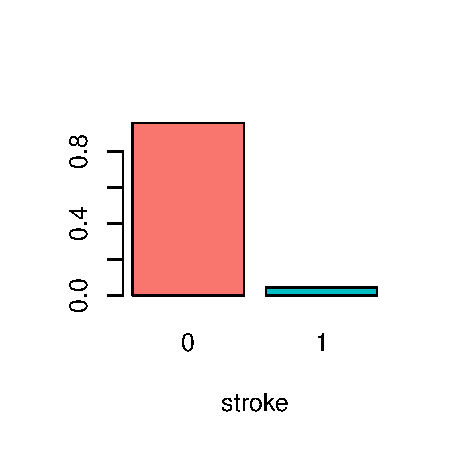
\includegraphics{stat-project-stroke_files/figure-latex/unnamed-chunk-7-1} \end{center}

These values are representative of the real situation in which there are
not many stroke cases compared with the whole population, the people who had a stroke are much less than the ones who did not have it. The
incidence of stroke in Europe at the beginning of the 21st century
varies from \(95\) to \(290\) cases/\(100,000\)\footnote{QUADERNI
  dell'Italian Journal of Medicine, A Journal of Hospital and Internal
  Medicine, Michele Meschi,volume 8, issue 2, March-April 2020}.
Furthermore in many clinical disease analyses this issue is commonly
present.

A visual transformation of the values seen in the \texttt{summary}
function is provided in the following boxplots:

\begin{Shaded}
\begin{Highlighting}[]
\FunctionTok{par}\NormalTok{(}\AttributeTok{mfrow=}\FunctionTok{c}\NormalTok{(}\DecValTok{1}\NormalTok{,}\DecValTok{3}\NormalTok{))}
\FunctionTok{boxplot}\NormalTok{(avg\_glucose\_level, }\AttributeTok{xlab=} \StringTok{\textquotesingle{}average glucose level\textquotesingle{}}\NormalTok{ , }\AttributeTok{col=}\StringTok{\textquotesingle{}\#00BA38\textquotesingle{}}\NormalTok{)}
\FunctionTok{boxplot}\NormalTok{(bmi, }\AttributeTok{xlab =} \StringTok{\textquotesingle{}body mass index\textquotesingle{}}\NormalTok{, }\AttributeTok{col=}\StringTok{\textquotesingle{}\#00BA38\textquotesingle{}}\NormalTok{)}
\FunctionTok{boxplot}\NormalTok{(age, }\AttributeTok{xlab =} \StringTok{\textquotesingle{}age\textquotesingle{}}\NormalTok{, }\AttributeTok{pch=}\DecValTok{20}\NormalTok{, }\AttributeTok{col=}\StringTok{\textquotesingle{}\#00BA38\textquotesingle{}}\NormalTok{)}
\end{Highlighting}
\end{Shaded}

\begin{figure}
\centering
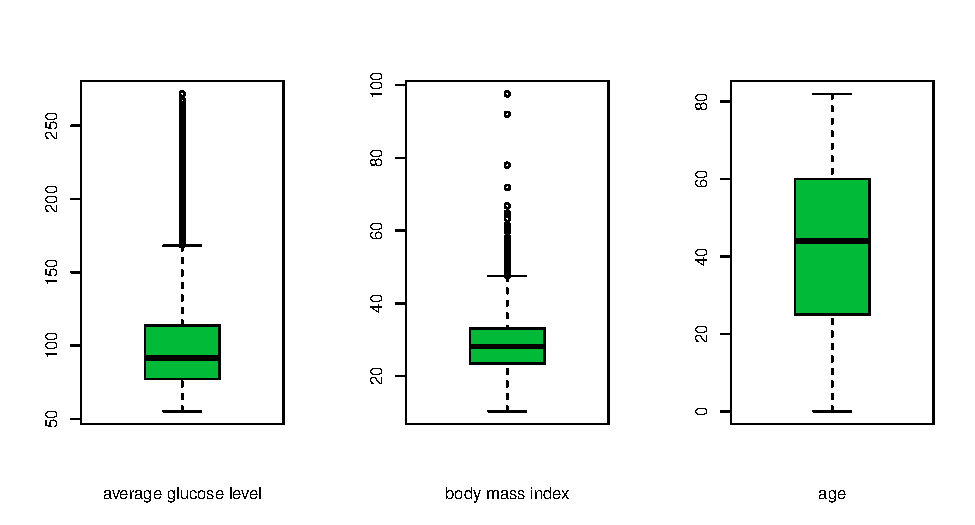
\includegraphics{stat-project-stroke_files/figure-latex/bp-1.pdf}
\caption{\label{bp}Visual description of some features of the dataset}
\end{figure}

\begin{Shaded}
\begin{Highlighting}[]
\FunctionTok{par}\NormalTok{(}\AttributeTok{mfrow=}\FunctionTok{c}\NormalTok{(}\DecValTok{1}\NormalTok{,}\DecValTok{1}\NormalTok{))}
\end{Highlighting}
\end{Shaded}

From Figure \ref{bp} we can see that in the first two boxplots (starting
from the left) there are lots of outliers for the variables
\texttt{avg\_glucose\_level} and \texttt{bmi}.\\
Actually, they represent real-case scenarios (people affected by high
glucose levels or with a bmi out of range are only a few) and possible
interesting cases of pathologies bounded with diabetes. Hence these data
points have to be considered during modeling, they will be helpful to
predict stroke cases because they could be due to complications of
diabetes disease, as mentioned in the medical literature.

In order to compare features in pairs and judge which one is
preferred, or has a greater amount of some quantitative property, we
provide a pair-wise plot. In addition, to involve also the categorical
variables we wrote some useful functions:

\begin{Shaded}
\begin{Highlighting}[]
\NormalTok{panel.cor }\OtherTok{\textless{}{-}} \ControlFlowTok{function}\NormalTok{(x, y, }\AttributeTok{digits =} \DecValTok{2}\NormalTok{, }\AttributeTok{prefix =} \StringTok{""}\NormalTok{, cex.cor, ...)\{}
\NormalTok{  usr }\OtherTok{\textless{}{-}} \FunctionTok{par}\NormalTok{(}\StringTok{"usr"}\NormalTok{); }\FunctionTok{on.exit}\NormalTok{(}\FunctionTok{par}\NormalTok{(usr))}
  \FunctionTok{par}\NormalTok{(}\AttributeTok{usr =} \FunctionTok{c}\NormalTok{(}\DecValTok{0}\NormalTok{, }\DecValTok{1}\NormalTok{, }\DecValTok{0}\NormalTok{, }\DecValTok{1}\NormalTok{))}
\NormalTok{  r }\OtherTok{\textless{}{-}} \FunctionTok{abs}\NormalTok{(}\FunctionTok{cor}\NormalTok{(x, y))}
\NormalTok{  txt }\OtherTok{\textless{}{-}} \FunctionTok{format}\NormalTok{(}\FunctionTok{c}\NormalTok{(r, }\FloatTok{0.123456789}\NormalTok{), }\AttributeTok{digits =}\NormalTok{ digits)[}\DecValTok{1}\NormalTok{]}
\NormalTok{  txt }\OtherTok{\textless{}{-}} \FunctionTok{paste0}\NormalTok{(prefix, txt)}
  \ControlFlowTok{if}\NormalTok{(}\FunctionTok{missing}\NormalTok{(cex.cor)) cex.cor }\OtherTok{\textless{}{-}} \FloatTok{0.8}\SpecialCharTok{/}\FunctionTok{strwidth}\NormalTok{(txt)}
  \FunctionTok{text}\NormalTok{(}\FloatTok{0.5}\NormalTok{, }\FloatTok{0.5}\NormalTok{, txt, }\AttributeTok{cex =}\NormalTok{ cex.cor }\SpecialCharTok{*}\NormalTok{ r)}
\NormalTok{\}}
\NormalTok{panel.hist }\OtherTok{\textless{}{-}} \ControlFlowTok{function}\NormalTok{(x, ...)}
\NormalTok{\{}
\NormalTok{  usr }\OtherTok{\textless{}{-}} \FunctionTok{par}\NormalTok{(}\StringTok{"usr"}\NormalTok{); }\FunctionTok{on.exit}\NormalTok{(}\FunctionTok{par}\NormalTok{(usr))}
  \FunctionTok{par}\NormalTok{(}\AttributeTok{usr =} \FunctionTok{c}\NormalTok{(usr[}\DecValTok{1}\SpecialCharTok{:}\DecValTok{2}\NormalTok{], }\DecValTok{0}\NormalTok{, }\FloatTok{1.5}\NormalTok{) )}
\NormalTok{  h }\OtherTok{\textless{}{-}} \FunctionTok{hist}\NormalTok{(x, }\AttributeTok{plot =} \ConstantTok{FALSE}\NormalTok{)}
\NormalTok{  breaks }\OtherTok{\textless{}{-}}\NormalTok{ h}\SpecialCharTok{$}\NormalTok{breaks; nB }\OtherTok{\textless{}{-}} \FunctionTok{length}\NormalTok{(breaks)}
\NormalTok{  y }\OtherTok{\textless{}{-}}\NormalTok{ h}\SpecialCharTok{$}\NormalTok{counts; y }\OtherTok{\textless{}{-}}\NormalTok{ y}\SpecialCharTok{/}\FunctionTok{max}\NormalTok{(y)}
  \FunctionTok{rect}\NormalTok{(breaks[}\SpecialCharTok{{-}}\NormalTok{nB], }\DecValTok{0}\NormalTok{, breaks[}\SpecialCharTok{{-}}\DecValTok{1}\NormalTok{], y, }\AttributeTok{col =} \StringTok{"green"}\NormalTok{, ...)}
\NormalTok{\}}
\end{Highlighting}
\end{Shaded}

And here we show the results from the pairs plot:

\begin{Shaded}
\begin{Highlighting}[]
\FunctionTok{pairs}\NormalTok{(stroke\_data, }\AttributeTok{diag.panel =}\NormalTok{ panel.hist, }\AttributeTok{upper.panel =}\NormalTok{ panel.cor)}
\end{Highlighting}
\end{Shaded}

\includegraphics{stat-project-stroke_files/figure-latex/unnamed-chunk-9-1.pdf}

The pairs-plot shows that the stronger relationships involve quite often
the variable \texttt{age}. But there are other small relevant relations,
for example between \texttt{work\_type} and \texttt{ever\_married} or
between \texttt{bmi} and \texttt{work\_type}. In addition, we can see
strong collinearity among the variables \texttt{age},
\texttt{work\_type}, and \texttt{ever\_married}, this means that they
are closely related to each another. For this reason we get uncertainty
in the coefficient estimates and so we do not consider them together in
the fitting of the models.\\
We go on looking at some intuitive relationship of \texttt{stroke} with
\texttt{age}, \texttt{bmi} and \texttt{avg\_glucose\_level}:

\begin{Shaded}
\begin{Highlighting}[]
\FunctionTok{par}\NormalTok{(}\AttributeTok{mfrow=}\FunctionTok{c}\NormalTok{(}\DecValTok{1}\NormalTok{,}\DecValTok{3}\NormalTok{))}
\FunctionTok{boxplot}\NormalTok{(avg\_glucose\_level}\SpecialCharTok{\textasciitilde{}}\NormalTok{stroke, }\AttributeTok{xlab =} \StringTok{\textquotesingle{}stroke\textquotesingle{}}\NormalTok{, }
        \AttributeTok{ylab =} \StringTok{\textquotesingle{}average glucose level\textquotesingle{}}\NormalTok{, }\AttributeTok{col =} \FunctionTok{c}\NormalTok{(}\StringTok{\textquotesingle{}\#F8766D\textquotesingle{}}\NormalTok{,}\StringTok{\textquotesingle{}\#00BFC4\textquotesingle{}}\NormalTok{))}
\FunctionTok{boxplot}\NormalTok{(bmi}\SpecialCharTok{\textasciitilde{}}\NormalTok{stroke, }\AttributeTok{xlab =} \StringTok{\textquotesingle{}stroke\textquotesingle{}}\NormalTok{, }\AttributeTok{ylab =} \StringTok{\textquotesingle{}bmi\textquotesingle{}}\NormalTok{, }\AttributeTok{col =} \FunctionTok{c}\NormalTok{(}\StringTok{\textquotesingle{}\#F8766D\textquotesingle{}}\NormalTok{,}\StringTok{\textquotesingle{}\#00BFC4\textquotesingle{}}\NormalTok{))}
\FunctionTok{boxplot}\NormalTok{(age}\SpecialCharTok{\textasciitilde{}}\NormalTok{stroke, }\AttributeTok{xlab =} \StringTok{\textquotesingle{}stroke\textquotesingle{}}\NormalTok{ , }\AttributeTok{ylab =} \StringTok{\textquotesingle{}age\textquotesingle{}}\NormalTok{, }\AttributeTok{col =} \FunctionTok{c}\NormalTok{(}\StringTok{\textquotesingle{}\#F8766D\textquotesingle{}}\NormalTok{,}\StringTok{\textquotesingle{}\#00BFC4\textquotesingle{}}\NormalTok{))}
\end{Highlighting}
\end{Shaded}

\begin{figure}
\centering
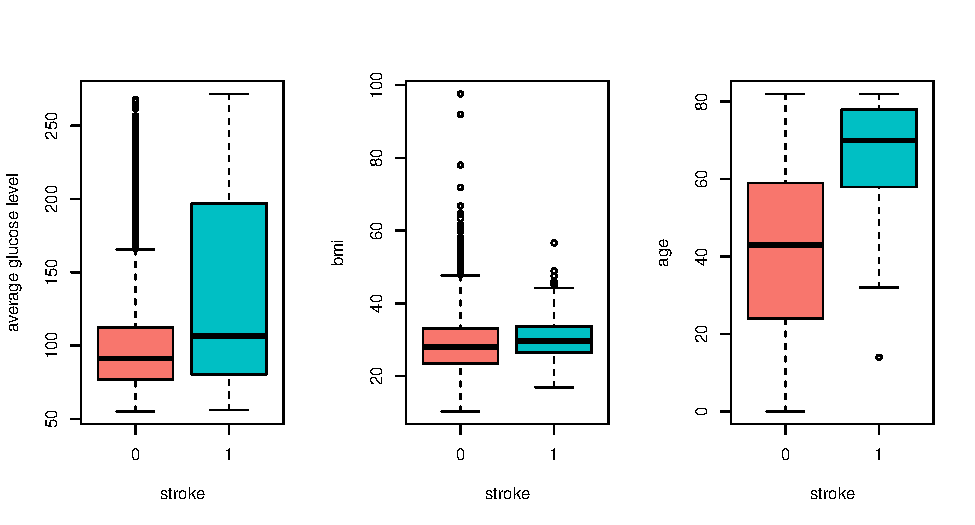
\includegraphics{stat-project-stroke_files/figure-latex/bp_stroke-1.pdf}
\caption{\label{bp_stroke}Visual rappresentation of the comparison
between \texttt{stroke}(1) and not-\texttt{stroke}(0) of the features:
\texttt{avg\_glucose\_level}, \texttt{bmi} and \texttt{age}.}
\end{figure}

\begin{Shaded}
\begin{Highlighting}[]
\FunctionTok{par}\NormalTok{(}\AttributeTok{mfrow=}\FunctionTok{c}\NormalTok{(}\DecValTok{1}\NormalTok{,}\DecValTok{1}\NormalTok{))}
\end{Highlighting}
\end{Shaded}

Looking at Figure \ref{bp_stroke} we can see that the incidence of the
disease increases progressively with age, in particular the summary of
\texttt{age} shows that the data observed cover people of all ages from
babies of 8 days to seniors of 82 years old (this can also be seen from the boxplot). We get also the information that the youngest person
affected of stroke disease has 14 years old (an outlier), while the
oldest one has 82 years old.\\
We make a more detailed analysis looking at the following tables:

\begin{Shaded}
\begin{Highlighting}[]
\FunctionTok{table}\NormalTok{(stroke.less}\FloatTok{.35} \OtherTok{\textless{}{-}}\NormalTok{ stroke\_data[stroke\_data}\SpecialCharTok{$}\NormalTok{age}\SpecialCharTok{\textless{}}\DecValTok{35}\NormalTok{, }\StringTok{\textquotesingle{}stroke\textquotesingle{}}\NormalTok{])}
\end{Highlighting}
\end{Shaded}

\begin{verbatim}
## 
##    0    1 
## 1796    2
\end{verbatim}

\begin{Shaded}
\begin{Highlighting}[]
\FunctionTok{table}\NormalTok{(stroke.}\FloatTok{35.50} \OtherTok{\textless{}{-}}\NormalTok{ stroke\_data[stroke\_data}\SpecialCharTok{$}\NormalTok{age}\SpecialCharTok{\textgreater{}=}\DecValTok{35} \SpecialCharTok{\&}\NormalTok{ stroke\_data}\SpecialCharTok{$}\NormalTok{age}\SpecialCharTok{\textless{}}\DecValTok{50}\NormalTok{ , }\StringTok{\textquotesingle{}stroke\textquotesingle{}}\NormalTok{])}
\end{Highlighting}
\end{Shaded}

\begin{verbatim}
## 
##    0    1 
## 1005   16
\end{verbatim}

\begin{Shaded}
\begin{Highlighting}[]
\FunctionTok{table}\NormalTok{(stroke.major}\FloatTok{.50} \OtherTok{\textless{}{-}}\NormalTok{ stroke\_data[stroke\_data}\SpecialCharTok{$}\NormalTok{age}\SpecialCharTok{\textgreater{}=}\DecValTok{50}\NormalTok{ , }\StringTok{\textquotesingle{}stroke\textquotesingle{}}\NormalTok{])}
\end{Highlighting}
\end{Shaded}

\begin{verbatim}
## 
##    0    1 
## 1899  191
\end{verbatim}

In \texttt{stroke.less.35} we can notice that there are only two people
under the age of 35 which have been affected by stroke, while in
\texttt{stroke.35.50} variable we highlight the number of people between the age
of 35 and 50 that are ill, i.e.~16. The major difference in the numbers
can be seen in \texttt{stroke.major.50} where stroke patients older than
50 are much more than the previous cases.\\
In Figure \ref{bp_stroke}, if we sum to \texttt{age} the information
about \texttt{avg\_glucose\_level} we may wonder if diabetic people are
more probable to get a stroke or not (first boxplot from the left). On
the other hand, there is no apparent relation of \texttt{stroke} with
\texttt{bmi} (central boxplot).

We now highlight other visual relationship between the variables used
before:

\begin{Shaded}
\begin{Highlighting}[]
\FunctionTok{library}\NormalTok{(ggplot2)}
\FunctionTok{ggplot}\NormalTok{(stroke\_data, }\FunctionTok{aes}\NormalTok{(}\AttributeTok{x =}\NormalTok{ avg\_glucose\_level, }\AttributeTok{y =}\NormalTok{ bmi, }\AttributeTok{col =} \FunctionTok{as.factor}\NormalTok{(stroke))) }\SpecialCharTok{+}
  \FunctionTok{labs}\NormalTok{(}\AttributeTok{x =} \StringTok{"average glucose level"}\NormalTok{, }\AttributeTok{y =} \StringTok{"bmi"}\NormalTok{, }\AttributeTok{color =} \StringTok{"Stroke"}\NormalTok{) }\SpecialCharTok{+} \FunctionTok{geom\_point}\NormalTok{()}
\end{Highlighting}
\end{Shaded}

\begin{center}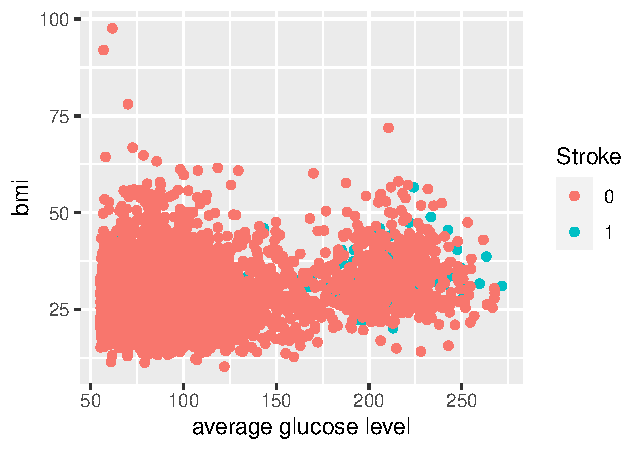
\includegraphics{stat-project-stroke_files/figure-latex/unnamed-chunk-11-1} \end{center}

\begin{Shaded}
\begin{Highlighting}[]
\FunctionTok{ggplot}\NormalTok{(stroke\_data, }\FunctionTok{aes}\NormalTok{(}\AttributeTok{x =}\NormalTok{ avg\_glucose\_level, }\AttributeTok{y =}\NormalTok{ age,}\AttributeTok{col =} \FunctionTok{as.factor}\NormalTok{(stroke))) }\SpecialCharTok{+} 
  \FunctionTok{labs}\NormalTok{(}\AttributeTok{x =} \StringTok{"average glucose level"}\NormalTok{, }\AttributeTok{y =} \StringTok{"age"}\NormalTok{, }\AttributeTok{color =} \StringTok{"Stroke"}\NormalTok{) }\SpecialCharTok{+} \FunctionTok{geom\_point}\NormalTok{()}
\end{Highlighting}
\end{Shaded}

\begin{center}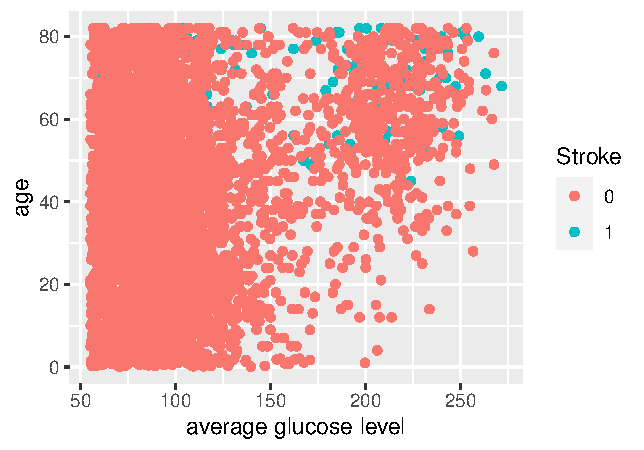
\includegraphics{stat-project-stroke_files/figure-latex/unnamed-chunk-11-2} \end{center}

\begin{Shaded}
\begin{Highlighting}[]
\FunctionTok{ggplot}\NormalTok{(stroke\_data, }\FunctionTok{aes}\NormalTok{(}\AttributeTok{x =}\NormalTok{ bmi, }\AttributeTok{y =}\NormalTok{ age, }\AttributeTok{col =} \FunctionTok{as.factor}\NormalTok{(stroke))) }\SpecialCharTok{+}
  \FunctionTok{labs}\NormalTok{(}\AttributeTok{x =} \StringTok{"bmi"}\NormalTok{, }\AttributeTok{y =} \StringTok{"age"}\NormalTok{, }\AttributeTok{color =} \StringTok{"Stroke"}\NormalTok{) }\SpecialCharTok{+} \FunctionTok{geom\_point}\NormalTok{()}
\end{Highlighting}
\end{Shaded}

\begin{center}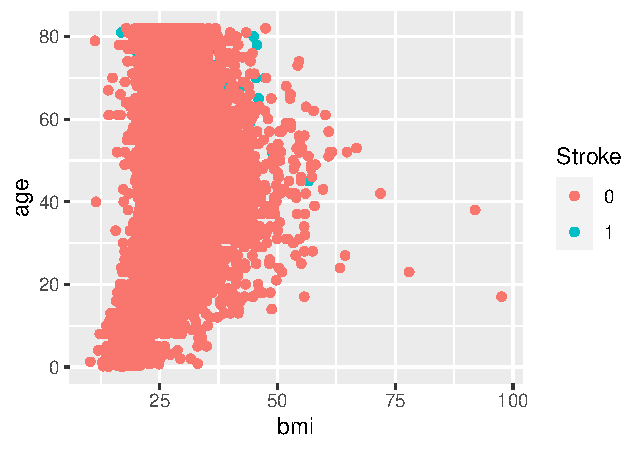
\includegraphics{stat-project-stroke_files/figure-latex/unnamed-chunk-11-3} \end{center}

What we can see from these scatter plots is that if we have low
\texttt{avg\_glucose\_level} values in relation with \texttt{age} or
\texttt{bmi}, the stroke disease tends to be not present. On the other
hand, if we look at the \texttt{bmi} predictor we can notice that there
are samples of stroke cases spread all over in all of its range of
values, so it highlights no clear correlation of \texttt{bmi} with
stroke, even when we put this features in relation with the others.\\
\texttt{avg\_glucose\_level} and \texttt{bmi} could not be so strictly
related to the disease but maybe correlated to other illnesses linked
(or not) to it.\\
In the end we can see that it is not easy to identify the direct
relationship with the stroke while dealing with the features that we
have, and it is difficult a further interpretation of the data.

\hypertarget{data-science-questions}{%
\subsection{2.3 Data Science Questions}\label{data-science-questions}}

At this point we can ask some questions:

\begin{itemize}
\tightlist
\item
  Which factors are the most related to the stroke disease?
\item
  How strong are the relations between the features?
\item
  Are the given variables enough to predict a good accuracy of some
  possible person affected by stroke?
\item
  Is it possible to prevent it?
\end{itemize}

We will explore the data trying to answer these questions.

\hypertarget{modeling}{%
\section{3 Modeling}\label{modeling}}

In order to explore different approaches for predicting the qualitative
response \texttt{stroke}, in the following paragraph we will cover three
of the most widely-used classifiers: \emph{logistic regression},
\emph{linear discriminant analysis (LDA)} and \emph{quadratic
discriminant analysis (QDA)}. The prediction process is known as
\emph{classification}.

\hypertarget{logistic-regression}{%
\subsection{3.1 Logistic Regression}\label{logistic-regression}}

Logistic regression can be defined as a type of \emph{generalized linear
model (GLM)}. In particular, it is a statistical model used to examine
the association of categorical or continuous independent variables with
one dichotomous dependent variable.\\
Rather than computing directly the response \(Y\), logistic regression
computes the probability that \(Y\) belongs to a particular category, in
our case \(1\) if the person has a stroke disease, \(0\) otherwise. In particular, to avoid predictions smaller than \(0\) or greater than \(1\) we use the \textit{logistic function},
\[ p(X) = \frac{e^{\beta_0 + \beta_1 X_1 + \dots + \beta_pX_p}}{1+e^{\beta_0 + \beta_1 X_1+ \dots + \beta_pX_p}}\]
with $p$ predictors.\\
In this part of the predictive analysis we will present three different
type of models, compared to discover the best one that can better
interpret the data. In particular, our model selection will be guide
both from the p-values and probabilistic statistical measure that
attempts to quantify both the model performance on the training dataset
and the complexity of the model. An example of this last strategy is
given by the \emph{Akaike Information Criterion (\(AIC\))}.\\
Compared with the \(BIC\) method, the \(AIC\) statistic penalizes
complex model less, meaning that it may put more emphasis on model
performance on the training dataset, and, in turn, select more complex
models. Its description is given by the following formula
\[ AIC = -2 \cdot \ell(\hat \Theta ) + 2d,\] where
\(\ell(\hat \Theta )\) is the maximized value of the log-likelihood
function for the estimated model and \(d\) the number of predictors. We
decided to exclude the Mallow's \(C_p\) and the \(R^2\) adjusted
techniques because they work efficiently in the case of linear
regression and not for logistic model.

\hypertarget{full-and-reduced-models}{%
\subsubsection{3.1.1 Full and Reduced
Models}\label{full-and-reduced-models}}

We start with the full model to see if all the features of the dataset
contribute on the prediction of a stroke.\\
Up to now we have already mentioned if some predictors seem to be more
or less correlated to the response variable, and a way to analyze such
relation is by introducing the \emph{null hypothesis}. In the case of
the full model, we are dealing with \(10\) explanatory variables and so
we have \[H_0 : \beta_1 = \dots = \beta_{10} = 0,\] and this means that
we are making the assumption that no predictors is somehow related with
\texttt{stroke}. If we reject the null hypothesis we are assuming that
there is in fact a correlation and we have to find which feature is
involved.\\
To decide whether or not reject \(H_0\) we set the alpha value to
\(\alpha = 0.1\) in order to decide whether a test statistic is
statistically significant, thus for p-values smaller than \(\alpha\) we
keep the feature otherwise we remove it from the model.\\
Let's have a look now at the characteristics of the full model:

\begin{Shaded}
\begin{Highlighting}[]
\NormalTok{mod.full }\OtherTok{\textless{}{-}} \FunctionTok{glm}\NormalTok{(stroke}\SpecialCharTok{\textasciitilde{}}\NormalTok{., }\AttributeTok{data =}\NormalTok{ stroke\_data, }\AttributeTok{family =}\NormalTok{ binomial)}
\FunctionTok{summary}\NormalTok{(mod.full)}
\end{Highlighting}
\end{Shaded}

\begin{verbatim}
## 
## Call:
## glm(formula = stroke ~ ., family = binomial, data = stroke_data)
## 
## Deviance Residuals: 
##     Min       1Q   Median       3Q      Max  
## -1.1823  -0.2947  -0.1524  -0.0744   3.5251  
## 
## Coefficients:
##                              Estimate Std. Error z value
## (Intercept)                -7.360e+00  1.067e+00  -6.895
## genderMale                 -1.463e-02  1.544e-01  -0.095
## genderOther                -1.135e+01  2.400e+03  -0.005
## age                         7.348e-02  6.347e-03  11.578
## hypertension                5.249e-01  1.750e-01   2.999
## heart_disease1              3.488e-01  2.072e-01   1.683
## ever_marriedYes            -1.152e-01  2.473e-01  -0.466
## work_typeGovt_job          -6.817e-01  1.114e+00  -0.612
## work_typeNever_worked      -1.082e+01  5.090e+02  -0.021
## work_typePrivate           -5.208e-01  1.100e+00  -0.473
## work_typeSelf-employed     -9.459e-01  1.119e+00  -0.845
## Residence_typeUrban         4.514e-03  1.500e-01   0.030
## avg_glucose_level           4.652e-03  1.294e-03   3.595
## bmi                         4.062e-03  1.188e-02   0.342
## smoking_statusnever smoked -6.722e-02  1.886e-01  -0.356
## smoking_statussmokes        3.139e-01  2.295e-01   1.368
## smoking_statusUnknown      -2.753e-01  2.471e-01  -1.114
##                            Pr(>|z|)    
## (Intercept)                5.37e-12 ***
## genderMale                 0.924525    
## genderOther                0.996225    
## age                         < 2e-16 ***
## hypertension               0.002711 ** 
## heart_disease1             0.092381 .  
## ever_marriedYes            0.641394    
## work_typeGovt_job          0.540660    
## work_typeNever_worked      0.983036    
## work_typePrivate           0.635943    
## work_typeSelf-employed     0.397906    
## Residence_typeUrban        0.975990    
## avg_glucose_level          0.000324 ***
## bmi                        0.732387    
## smoking_statusnever smoked 0.721556    
## smoking_statussmokes       0.171310    
## smoking_statusUnknown      0.265193    
## ---
## Signif. codes:  
## 0 '***' 0.001 '**' 0.01 '*' 0.05 '.' 0.1 ' ' 1
## 
## (Dispersion parameter for binomial family taken to be 1)
## 
##     Null deviance: 1728.4  on 4908  degrees of freedom
## Residual deviance: 1363.2  on 4892  degrees of freedom
## AIC: 1397.2
## 
## Number of Fisher Scoring iterations: 15
\end{verbatim}

Here we see that \texttt{age}, \texttt{avg\_glucose\_level} and
\texttt{hypertension} are the variables most related to \texttt{stroke},
with a p-value smaller than \(0.005\), but also \texttt{heart\_disease}
contributes a bit to the model with a p-value of \(0.092381\). As
expected, the collinearity factors, i.e.~\texttt{work\_type} and \texttt{ever\_married}, do not
contribute.\\
Let's use the residual plots to get more information about this model.

\begin{Shaded}
\begin{Highlighting}[]
\FunctionTok{par}\NormalTok{(}\AttributeTok{mfrow=}\FunctionTok{c}\NormalTok{(}\DecValTok{2}\NormalTok{,}\DecValTok{2}\NormalTok{))}
\FunctionTok{plot}\NormalTok{(mod.full)}
\end{Highlighting}
\end{Shaded}

\begin{verbatim}
## Warning: not plotting observations with leverage one:
##   2971
\end{verbatim}

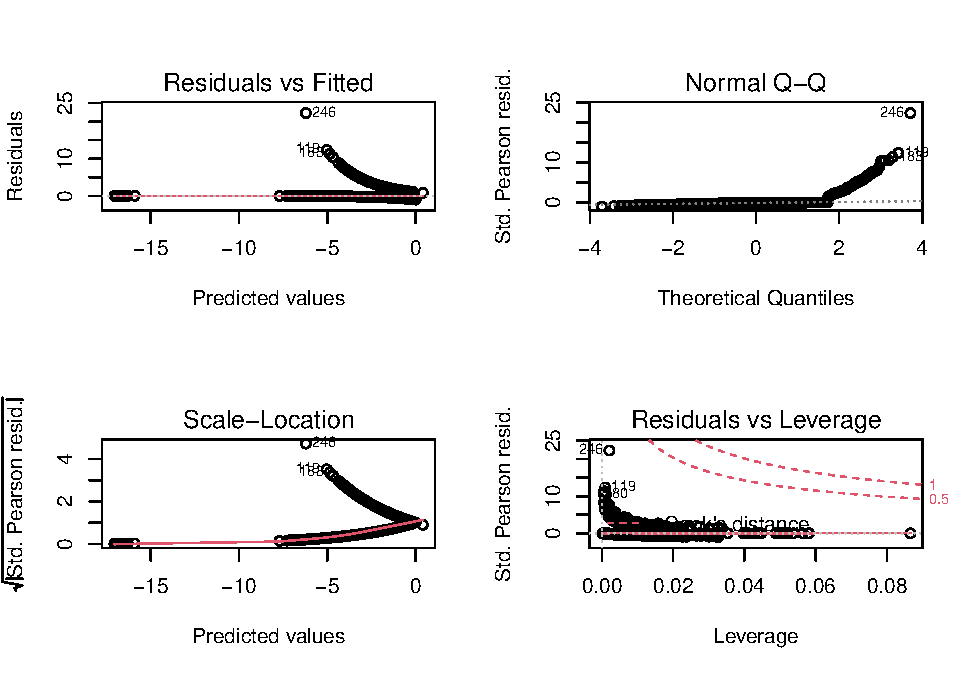
\includegraphics{stat-project-stroke_files/figure-latex/unnamed-chunk-13-1.pdf}

\begin{Shaded}
\begin{Highlighting}[]
\FunctionTok{par}\NormalTok{(}\AttributeTok{mfrow=}\FunctionTok{c}\NormalTok{(}\DecValTok{1}\NormalTok{,}\DecValTok{1}\NormalTok{))}
\end{Highlighting}
\end{Shaded}

The plots are not satisfactory because they are not easy to interpret.
It is simply evident that data do not follow a linear trend (we will
discuss more in detail in the next paragraphs).

We now go on with some tests, we take the full model and we remove all
the predictors that show up collinearity between each other, following a
sort of greedy backward selection:

\begin{Shaded}
\begin{Highlighting}[]
\NormalTok{mod.red1 }\OtherTok{\textless{}{-}} \FunctionTok{glm}\NormalTok{(stroke }\SpecialCharTok{\textasciitilde{}}\NormalTok{ age }\SpecialCharTok{+}\NormalTok{ bmi }\SpecialCharTok{+}\NormalTok{ avg\_glucose\_level }\SpecialCharTok{+}\NormalTok{ hypertension }\SpecialCharTok{+} 
\NormalTok{                  smoking\_status }\SpecialCharTok{+}\NormalTok{ gender }\SpecialCharTok{+}\NormalTok{ heart\_disease, }\AttributeTok{family =}\NormalTok{ binomial)}
\FunctionTok{summary}\NormalTok{(mod.red1)}
\end{Highlighting}
\end{Shaded}

\begin{verbatim}
## 
## Call:
## glm(formula = stroke ~ age + bmi + avg_glucose_level + hypertension + 
##     smoking_status + gender + heart_disease, family = binomial)
## 
## Deviance Residuals: 
##     Min       1Q   Median       3Q      Max  
## -1.0751  -0.2957  -0.1572  -0.0734   3.6706  
## 
## Coefficients:
##                              Estimate Std. Error z value
## (Intercept)                 -7.823946   0.588445 -13.296
## age                          0.069041   0.005847  11.808
## bmi                          0.003458   0.011745   0.294
## avg_glucose_level            0.004697   0.001289   3.644
## hypertension                 0.517649   0.174438   2.968
## smoking_statusnever smoked  -0.057792   0.187972  -0.307
## smoking_statussmokes         0.321264   0.228512   1.406
## smoking_statusUnknown       -0.256978   0.245259  -1.048
## genderMale                  -0.011195   0.154011  -0.073
## genderOther                 -7.287812 324.743860  -0.022
## heart_disease1               0.372836   0.206072   1.809
##                            Pr(>|z|)    
## (Intercept)                 < 2e-16 ***
## age                         < 2e-16 ***
## bmi                        0.768441    
## avg_glucose_level          0.000269 ***
## hypertension               0.003002 ** 
## smoking_statusnever smoked 0.758502    
## smoking_statussmokes       0.159754    
## smoking_statusUnknown      0.294740    
## genderMale                 0.942055    
## genderOther                0.982096    
## heart_disease1             0.070411 .  
## ---
## Signif. codes:  
## 0 '***' 0.001 '**' 0.01 '*' 0.05 '.' 0.1 ' ' 1
## 
## (Dispersion parameter for binomial family taken to be 1)
## 
##     Null deviance: 1728.4  on 4908  degrees of freedom
## Residual deviance: 1369.4  on 4898  degrees of freedom
## AIC: 1391.4
## 
## Number of Fisher Scoring iterations: 11
\end{verbatim}

Also in this case the more important covariates are the same of the ones
found in the full model.\\
In this step we remove the \texttt{gender} variable, because it is not
significant and we end up with more or less the same results as before.

\begin{Shaded}
\begin{Highlighting}[]
\NormalTok{mod.red2 }\OtherTok{\textless{}{-}} \FunctionTok{glm}\NormalTok{(stroke }\SpecialCharTok{\textasciitilde{}}\NormalTok{ age }\SpecialCharTok{+}\NormalTok{ bmi }\SpecialCharTok{+}\NormalTok{ avg\_glucose\_level }\SpecialCharTok{+}\NormalTok{ hypertension }\SpecialCharTok{+} 
\NormalTok{                  smoking\_status  }\SpecialCharTok{+}\NormalTok{ heart\_disease, }\AttributeTok{family =}\NormalTok{ binomial)}
\FunctionTok{summary}\NormalTok{(mod.red2)}
\end{Highlighting}
\end{Shaded}

\begin{verbatim}
## 
## Call:
## glm(formula = stroke ~ age + bmi + avg_glucose_level + hypertension + 
##     smoking_status + heart_disease, family = binomial)
## 
## Deviance Residuals: 
##     Min       1Q   Median       3Q      Max  
## -1.0766  -0.2964  -0.1572  -0.0733   3.6720  
## 
## Coefficients:
##                             Estimate Std. Error z value
## (Intercept)                -7.830942   0.582317 -13.448
## age                         0.069065   0.005842  11.822
## bmi                         0.003487   0.011744   0.297
## avg_glucose_level           0.004689   0.001285   3.648
## hypertension                0.517599   0.174427   2.967
## smoking_statusnever smoked -0.055884   0.186343  -0.300
## smoking_statussmokes        0.321811   0.228437   1.409
## smoking_statusUnknown      -0.255822   0.244827  -1.045
## heart_disease1              0.371145   0.204739   1.813
##                            Pr(>|z|)    
## (Intercept)                 < 2e-16 ***
## age                         < 2e-16 ***
## bmi                        0.766535    
## avg_glucose_level          0.000264 ***
## hypertension               0.003003 ** 
## smoking_statusnever smoked 0.764254    
## smoking_statussmokes       0.158907    
## smoking_statusUnknown      0.296066    
## heart_disease1             0.069867 .  
## ---
## Signif. codes:  
## 0 '***' 0.001 '**' 0.01 '*' 0.05 '.' 0.1 ' ' 1
## 
## (Dispersion parameter for binomial family taken to be 1)
## 
##     Null deviance: 1728.4  on 4908  degrees of freedom
## Residual deviance: 1369.4  on 4900  degrees of freedom
## AIC: 1387.4
## 
## Number of Fisher Scoring iterations: 7
\end{verbatim}

The parameters left to delete are \texttt{bmi} and
\texttt{smoking\_status} that continue to have a high p-value. 

\begin{Shaded}
\begin{Highlighting}[]
\NormalTok{mod.red }\OtherTok{\textless{}{-}} \FunctionTok{glm}\NormalTok{(stroke}\SpecialCharTok{\textasciitilde{}}\NormalTok{age }\SpecialCharTok{+}\NormalTok{ avg\_glucose\_level }\SpecialCharTok{+}\NormalTok{ heart\_disease }\SpecialCharTok{+}\NormalTok{ hypertension, }
               \AttributeTok{family =}\NormalTok{ binomial)}
\FunctionTok{summary}\NormalTok{(mod.red)}
\end{Highlighting}
\end{Shaded}

\begin{verbatim}
## 
## Call:
## glm(formula = stroke ~ age + avg_glucose_level + heart_disease + 
##     hypertension, family = binomial)
## 
## Deviance Residuals: 
##     Min       1Q   Median       3Q      Max  
## -1.0995  -0.2940  -0.1599  -0.0778   3.5885  
## 
## Coefficients:
##                    Estimate Std. Error z value Pr(>|z|)    
## (Intercept)       -7.660740   0.387152 -19.787  < 2e-16 ***
## age                0.067547   0.005571  12.124  < 2e-16 ***
## avg_glucose_level  0.004802   0.001255   3.828 0.000129 ***
## heart_disease1     0.404298   0.203447   1.987 0.046895 *  
## hypertension       0.539613   0.173055   3.118 0.001820 ** 
## ---
## Signif. codes:  
## 0 '***' 0.001 '**' 0.01 '*' 0.05 '.' 0.1 ' ' 1
## 
## (Dispersion parameter for binomial family taken to be 1)
## 
##     Null deviance: 1728.4  on 4908  degrees of freedom
## Residual deviance: 1374.6  on 4904  degrees of freedom
## AIC: 1384.6
## 
## Number of Fisher Scoring iterations: 7
\end{verbatim}

An important thing to notice is the decreasing p-value of the explanatory variable \texttt{heart\_disease}, that now is equal to \(0.046895\).

The final reduced model is then composed of four explanatory variables and this means that our logistic function becomes:
\[p(X)= \frac{e^{\beta_0+\beta_1X_1 + \beta_2X_2+\beta_3 X_3+\beta_4 X_4}}{1+e^{\beta_0+\beta_1X_1 + \beta_2X_2+\beta_3 X_3+\beta_4 X_4}},\]
where \(\beta_0, \dots, \beta_4\) can be read in the \texttt{summary} of
\texttt{mod.red}, as the coefficient estimates, with the respectively
variables \(X_1, \dots, X_4\) which represent \texttt{age},
\texttt{avg\_glucose\_level}, \texttt{heart\_disease} and
\texttt{hypertension}.\\
From \(p(X)\) we can get the quantity \(p(X)/(1-p(X))\) which is called
\emph{odds}, and it can take any value between \(0\) and \(\infty\).
Values of odds close to \(0\) and \(\infty\) indicates very low and very
high probabilities to get a stroke, respectively.\\
In our logistic regression model, increasing \(X_i\) by one unit
multiplies the odds by \(e^{\beta_i}\), for \(i=1, \dots, 4\). The
amount of change in \(p(X)\) due to a one-unit change in \(X_i\) depending
on the current value of \(X_i\). But regardless of the value of \(X_i\),
if \(\beta_i\) is positive than increasing \(X_i\) will be associated
with increasing \(p(X)\), and if \(\beta_i\) is negative than increasing
\(X_i\) will be associated with decreasing \(p(X)\), for
\(i=1, \dots, 4\).\\
The fact that there is not a straight-line relationship between \(p(X)\)
and \(X_i\), and the fact that the rate of change in \(p(X)\) per unit
change in \(X_i\) depends on the current value of \(X_i\).

For this model we also give a descriptive statistic through the residual
plots:

\begin{Shaded}
\begin{Highlighting}[]
\FunctionTok{par}\NormalTok{(}\AttributeTok{mfrow=}\FunctionTok{c}\NormalTok{(}\DecValTok{2}\NormalTok{,}\DecValTok{2}\NormalTok{))}
\FunctionTok{plot}\NormalTok{(mod.red)}
\end{Highlighting}
\end{Shaded}

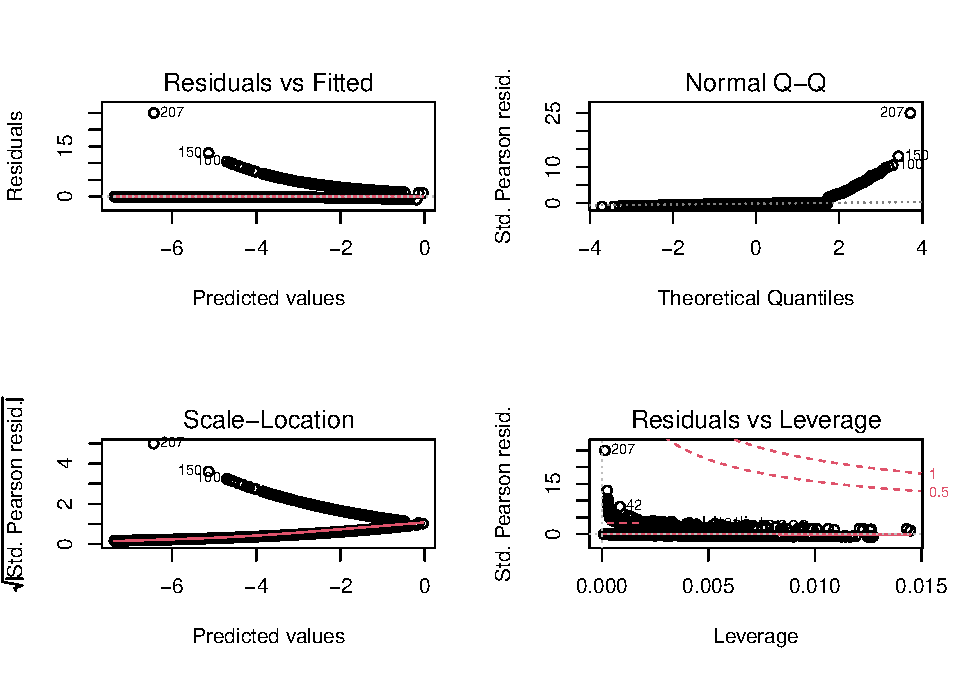
\includegraphics{stat-project-stroke_files/figure-latex/unnamed-chunk-17-1.pdf}

\begin{Shaded}
\begin{Highlighting}[]
\FunctionTok{par}\NormalTok{(}\AttributeTok{mfrow=}\FunctionTok{c}\NormalTok{(}\DecValTok{1}\NormalTok{,}\DecValTok{1}\NormalTok{))}
\end{Highlighting}
\end{Shaded}

Reading and interpreting these graphs, we can state some important
outcomes:

\textbf{Residuals vs Fitted}\\
We can observe the presence of high non-linearity in the dataset. Indeed
we can find not spread equal residuals around a horizontal line without
distinct patterns, attesting to the fact that there is no linear
relationship.

\textbf{Normal Q-Q}\\
We discover that residuals do not follow a normal distribution.\\
We know that obtaining positive coefficient estimates, we have a
positive association. So, the larger the value the higher is the
estimated probability of stroke.

\textbf{Scale-Location}\\
We can see that homoscedasticity does not hold since the line of the
standard residual is not flat, hence even by standardizing the residuals
we end up having high variance among them. But in our case, as you can
notice from this plot, the red line is slightly curved and the residuals
increase as the fitted \(Y\) value increases. So, the inference here
is, heteroscedasticity exists.

\textbf{Residual vs Leverage}\\
Looking at the leverage plot, we see the presence of some samples with
high leverage value (bottom right), which could influence the prediction
of the model (even if the R-plot does not show us its index).

Moreover, in Table \ref{outliers_reduced}, there are outliers (with no connection with our regression) that have high variance, and they represent some rare cases of disease development; as we saw previously there was a case
of a 14 years old girl that had stroke.


\begin{longtable}[]{@{}lccccccccccc@{}}
\toprule
& gender & age & hypert. & hd & ev\_marr & work\_type & res\_type &
glucose & bmi & smoking & stroke \\
\midrule
\endhead
119 & Female & 38 & 0 & 0 & No & Self-employed & Urban & 82.28 & 24.0 &
formerly smoked & 1 \\
183 & Female & 32 & 0 & 0 & Yes & Private & Rural & 76.13 & 29.9 &
smokes & 1 \\
246 & Female & 14 & 0 & 0 & No & children & Rural & 57.93 & 30.9 &
Unknown & 1 \\
\bottomrule
\caption{Outliers of the Reduced Model}\label{outliers_reduced}
\end{longtable}
If we look at the results, we can affirm that the reduced model seems to make a more accurate prediction and fits better data than the full one. Indeed, its \(AIC\)
is the lowest of the two.\\
To have a confirmation of this result we used \texttt{anova}, a function
which allows us to provide a comparison. The null hypothesis is that the
two models fit the data equally well, and the alternative hypothesis is
that the reduced model is superior.

\begin{Shaded}
\begin{Highlighting}[]
\FunctionTok{anova}\NormalTok{(mod.red, mod.full, }\AttributeTok{test=}\StringTok{"Chisq"}\NormalTok{)}
\end{Highlighting}
\end{Shaded}

\begin{verbatim}
## Analysis of Deviance Table
## 
## Model 1: stroke ~ age + avg_glucose_level + heart_disease + hypertension
## Model 2: stroke ~ gender + age + hypertension + heart_disease + ever_married + 
##     work_type + Residence_type + avg_glucose_level + bmi + smoking_status
##   Resid. Df Resid. Dev Df Deviance Pr(>Chi)
## 1      4904     1374.7                     
## 2      4892     1363.2 12    11.42   0.4933
\end{verbatim}

As we know, the \texttt{anova} table gives us the deviance difference,
the degrees of freedom and above all the statistical test. As expected,
the anova test rejects that the full model is more pertinent than the
reduced one, since the p-value of its features are not less than \(5\%\)
or even \(10\%\). Therefore the full model does not enhance the
prediction.

\hypertarget{interaction-models}{%
\subsubsection{3.1.2 Interaction Models}\label{interaction-models}}

Let's try to check other convenient models using a mixed approach. We
use the reduced model \texttt{mod.red} as landmark and we proceed with
interactions between the explanatory variables with the aim to
understand which variables are relevant on our research and to improve
the performance of the model. We recall that we defined the significance levels equal to \(0.1\) and we will look for an \(AIC\) value lower than previous seen.\\
The model \texttt{mod.red} has \texttt{stroke} as response and
\texttt{age}, \texttt{avg\_glucose\_level}, \texttt{hypertension} and
\texttt{heart\_disease} as predictors, and with \(AIC\) of
\(1384.6\).

Initially we consider the interaction of \texttt{age} with the other
numerical features, i.e.~\texttt{avg\_glucose\_level},
\texttt{hypertension} and \texttt{heart\_disease} and we achive that
only \texttt{age*heart\_disease} gives a relevant contribution. We get
\(AIC = 1384\).

\begin{Shaded}
\begin{Highlighting}[]
\NormalTok{mod1 }\OtherTok{\textless{}{-}} \FunctionTok{glm}\NormalTok{(stroke }\SpecialCharTok{\textasciitilde{}}\NormalTok{ age }\SpecialCharTok{+}\NormalTok{ avg\_glucose\_level }\SpecialCharTok{+}\NormalTok{ heart\_disease }\SpecialCharTok{+}\NormalTok{ hypertension }\SpecialCharTok{+}
\NormalTok{               age}\SpecialCharTok{*}\NormalTok{heart\_disease, }\AttributeTok{family=}\NormalTok{binomial)}
\FunctionTok{summary}\NormalTok{(mod1)}
\end{Highlighting}
\end{Shaded}

\begin{verbatim}
## 
## Call:
## glm(formula = stroke ~ age + avg_glucose_level + heart_disease + 
##     hypertension + age * heart_disease, family = binomial)
## 
## Deviance Residuals: 
##     Min       1Q   Median       3Q      Max  
## -0.9897  -0.2980  -0.1557  -0.0737   3.6232  
## 
## Coefficients:
##                     Estimate Std. Error z value Pr(>|z|)    
## (Intercept)        -7.816578   0.407175 -19.197  < 2e-16 ***
## age                 0.070133   0.005889  11.908  < 2e-16 ***
## avg_glucose_level   0.004702   0.001253   3.752 0.000176 ***
## heart_disease1      2.765299   1.396557   1.980 0.047694 *  
## hypertension        0.536550   0.172602   3.109 0.001880 ** 
## age:heart_disease1 -0.032872   0.019486  -1.687 0.091604 .  
## ---
## Signif. codes:  
## 0 '***' 0.001 '**' 0.01 '*' 0.05 '.' 0.1 ' ' 1
## 
## (Dispersion parameter for binomial family taken to be 1)
## 
##     Null deviance: 1728.4  on 4908  degrees of freedom
## Residual deviance: 1372.0  on 4903  degrees of freedom
## AIC: 1384
## 
## Number of Fisher Scoring iterations: 7
\end{verbatim}

Furthermore, we can see that the interaction variable is statistically
significant for an alpha value set to 0.1, hence we can say that the two
slopes for the two different groups, affected by the heart disease and
not, are significantly different to each other. Last but not least, we
saw that by considering the interaction we have also a high increment in
the beta value of the heart disease.

After considerating all the interaction of \texttt{avg\_glucose\_level} with
the remaining predictors we find out that
\texttt{avg\_glucose\_level*hypertension} is the best of the possible
relations even if it can not improve the previous models.\\
It has an \(AIC\) of \(1385.9\).

\begin{Shaded}
\begin{Highlighting}[]
\NormalTok{mod2 }\OtherTok{\textless{}{-}} \FunctionTok{glm}\NormalTok{(stroke }\SpecialCharTok{\textasciitilde{}}\NormalTok{ age }\SpecialCharTok{+}\NormalTok{ avg\_glucose\_level }\SpecialCharTok{+}\NormalTok{ heart\_disease }\SpecialCharTok{+}\NormalTok{ hypertension }\SpecialCharTok{+}
\NormalTok{              avg\_glucose\_level}\SpecialCharTok{*}\NormalTok{hypertension, }\AttributeTok{family=}\NormalTok{binomial)}
\FunctionTok{summary}\NormalTok{(mod2)}
\end{Highlighting}
\end{Shaded}

\begin{verbatim}
## 
## Call:
## glm(formula = stroke ~ age + avg_glucose_level + heart_disease + 
##     hypertension + avg_glucose_level * hypertension, family = binomial)
## 
## Deviance Residuals: 
##     Min       1Q   Median       3Q      Max  
## -1.0453  -0.2958  -0.1590  -0.0775   3.5977  
## 
## Coefficients:
##                                 Estimate Std. Error z value
## (Intercept)                    -7.731877   0.395629 -19.543
## age                             0.067246   0.005586  12.038
## avg_glucose_level               0.005525   0.001484   3.723
## heart_disease1                  0.401439   0.203302   1.975
## hypertension                    0.877774   0.413934   2.121
## avg_glucose_level:hypertension -0.002413   0.002710  -0.890
##                                Pr(>|z|)    
## (Intercept)                     < 2e-16 ***
## age                             < 2e-16 ***
## avg_glucose_level              0.000197 ***
## heart_disease1                 0.048314 *  
## hypertension                   0.033958 *  
## avg_glucose_level:hypertension 0.373262    
## ---
## Signif. codes:  
## 0 '***' 0.001 '**' 0.01 '*' 0.05 '.' 0.1 ' ' 1
## 
## (Dispersion parameter for binomial family taken to be 1)
## 
##     Null deviance: 1728.4  on 4908  degrees of freedom
## Residual deviance: 1373.9  on 4903  degrees of freedom
## AIC: 1385.9
## 
## Number of Fisher Scoring iterations: 7
\end{verbatim}

Ultimately, we have the interaction \texttt{heart\_disease*hypertension}
which shows a good model with \(AIC = 1384.5\).

\begin{Shaded}
\begin{Highlighting}[]
\NormalTok{mod3 }\OtherTok{\textless{}{-}} \FunctionTok{glm}\NormalTok{(stroke }\SpecialCharTok{\textasciitilde{}}\NormalTok{ age }\SpecialCharTok{+}\NormalTok{ avg\_glucose\_level }\SpecialCharTok{+}\NormalTok{ heart\_disease }\SpecialCharTok{+}\NormalTok{ hypertension }\SpecialCharTok{+} 
\NormalTok{            heart\_disease}\SpecialCharTok{*}\NormalTok{hypertension, }\AttributeTok{family =}\NormalTok{ binomial)}
\FunctionTok{summary}\NormalTok{(mod3)}
\end{Highlighting}
\end{Shaded}

\begin{verbatim}
## 
## Call:
## glm(formula = stroke ~ age + avg_glucose_level + heart_disease + 
##     hypertension + heart_disease * hypertension, family = binomial)
## 
## Deviance Residuals: 
##     Min       1Q   Median       3Q      Max  
## -1.0079  -0.2951  -0.1584  -0.0774   3.5900  
## 
## Coefficients:
##                              Estimate Std. Error z value
## (Intercept)                 -7.657815   0.387787 -19.747
## age                          0.067108   0.005592  12.001
## avg_glucose_level            0.004760   0.001256   3.791
## heart_disease1               0.592399   0.236015   2.510
## hypertension                 0.660347   0.189663   3.482
## heart_disease1:hypertension -0.635251   0.444325  -1.430
##                             Pr(>|z|)    
## (Intercept)                  < 2e-16 ***
## age                          < 2e-16 ***
## avg_glucose_level           0.000150 ***
## heart_disease1              0.012073 *  
## hypertension                0.000498 ***
## heart_disease1:hypertension 0.152803    
## ---
## Signif. codes:  
## 0 '***' 0.001 '**' 0.01 '*' 0.05 '.' 0.1 ' ' 1
## 
## (Dispersion parameter for binomial family taken to be 1)
## 
##     Null deviance: 1728.4  on 4908  degrees of freedom
## Residual deviance: 1372.5  on 4903  degrees of freedom
## AIC: 1384.5
## 
## Number of Fisher Scoring iterations: 7
\end{verbatim}

After that, we picked up the reduced model without \texttt{heart\_disease}
which represents the explanatory feature with higher p-value and we
continued to work in the same way we have just seen. We repeated the
scheme with \texttt{age}, without earning benefits.\\
The \(AIC\) has a value of \(1386.2\).

\begin{Shaded}
\begin{Highlighting}[]
\NormalTok{mod4 }\OtherTok{\textless{}{-}} \FunctionTok{glm}\NormalTok{(stroke }\SpecialCharTok{\textasciitilde{}}\NormalTok{ age }\SpecialCharTok{+}\NormalTok{ avg\_glucose\_level }\SpecialCharTok{+}\NormalTok{ hypertension }\SpecialCharTok{+}\NormalTok{ age}\SpecialCharTok{*}\NormalTok{hypertension,}
              \AttributeTok{family=}\NormalTok{binomial)}
\end{Highlighting}
\end{Shaded}

We go further analyzing also \texttt{avg\_glucose\_level*hypertension}.

\begin{Shaded}
\begin{Highlighting}[]
\NormalTok{mod5 }\OtherTok{\textless{}{-}} \FunctionTok{glm}\NormalTok{(stroke }\SpecialCharTok{\textasciitilde{}}\NormalTok{ age }\SpecialCharTok{+}\NormalTok{ avg\_glucose\_level }\SpecialCharTok{+}\NormalTok{ hypertension }\SpecialCharTok{+} 
\NormalTok{              avg\_glucose\_level}\SpecialCharTok{*}\NormalTok{hypertension, }\AttributeTok{family =}\NormalTok{ binomial)}
\end{Highlighting}
\end{Shaded}

In the end, we include the possible best interactions into the reduced
model. It could be a good way, but it does not represent our best
solution due to a high p-value.\\
The corresponding \(AIC\) is \(1384.2\).

\begin{Shaded}
\begin{Highlighting}[]
\NormalTok{mod6 }\OtherTok{\textless{}{-}} \FunctionTok{glm}\NormalTok{(stroke }\SpecialCharTok{\textasciitilde{}}\NormalTok{ age }\SpecialCharTok{+}\NormalTok{ avg\_glucose\_level }\SpecialCharTok{+}\NormalTok{ heart\_disease }\SpecialCharTok{+}\NormalTok{ hypertension }\SpecialCharTok{+}
\NormalTok{              age}\SpecialCharTok{*}\NormalTok{heart\_disease }\SpecialCharTok{+}\NormalTok{ heart\_disease}\SpecialCharTok{*}\NormalTok{hypertension, }\AttributeTok{family =}\NormalTok{ binomial)}
\end{Highlighting}
\end{Shaded}

As conclusion, we can promote \texttt{mod1} as the model which better
fits our data:
\[log\bigg(\frac{p(X)}{1-p(X)}\bigg) = \beta_0 + \beta_1\times \verb!age! + \beta_2\times \verb|avg_glucose_level| + \beta_3 \times \verb|heart_disease| \,+ \]
\[+\, \beta_4 \times\verb|hypertension| + \beta_5 \times \verb |age*heart_disease|\]

Let's now see some relevant information, such as outliers of
\texttt{mod1}, looking at Table \ref{outliers_mod1}:

\setlength\LTleft{-.5cm}
\begin{longtable}[]{@{}lccccccccccc@{}}
\toprule
& gender & age & hypert. & hd & ev\_marr & work\_type & res\_type &
glucose & bmi & smoking & stroke \\
\midrule
\endhead
207 & Female & 81 & 0 & 0 & Yes & Private & Rural & 80.13 & 23.4 & never
smoked & 1 \\
150 & Female & 70 & 0 & 1 & Yes & Private & Rural & 239.07 & 26.1 &
never smoked & 1 \\
100 & Female & 69 & 0 & 0 & Yes & Govt\_job & Urban & 82.81 & 28.0 &
never smoked & 1 \\
\bottomrule
\caption{Outliers of Interaction Model \texttt{mod1}}\label{outliers_mod1}
\end{longtable}

and other properties and characteristics by the plots:

\begin{Shaded}
\begin{Highlighting}[]
\FunctionTok{par}\NormalTok{(}\AttributeTok{mfrow=}\FunctionTok{c}\NormalTok{(}\DecValTok{2}\NormalTok{,}\DecValTok{2}\NormalTok{))}
\FunctionTok{plot}\NormalTok{(mod.full)}
\end{Highlighting}
\end{Shaded}

\begin{verbatim}
## Warning: not plotting observations with leverage one:
##   2971
\end{verbatim}

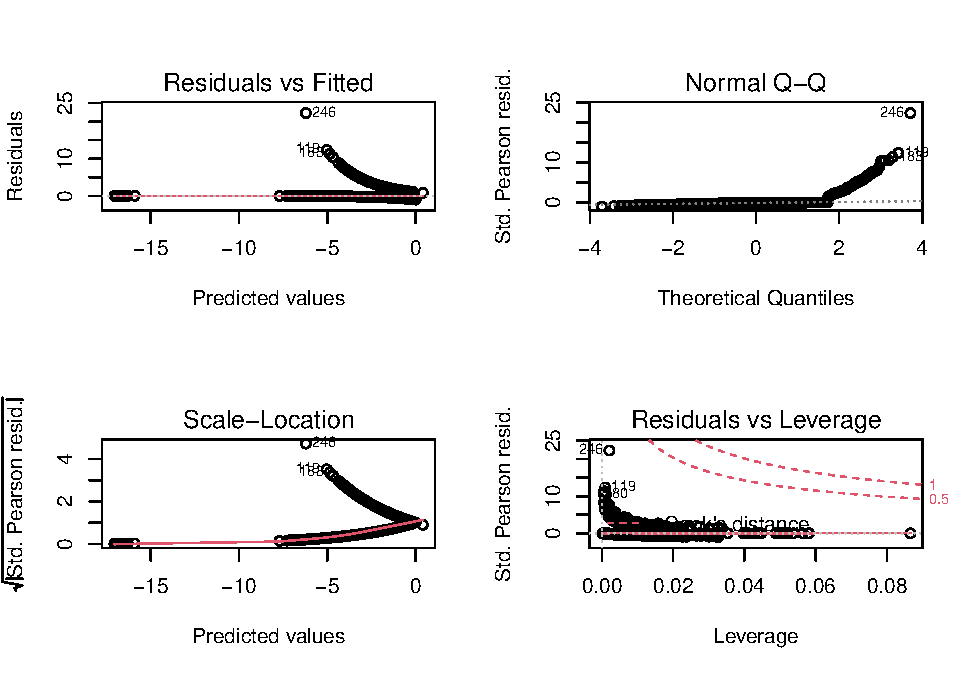
\includegraphics{stat-project-stroke_files/figure-latex/unnamed-chunk-27-1.pdf}

\begin{Shaded}
\begin{Highlighting}[]
\FunctionTok{par}\NormalTok{(}\AttributeTok{mfrow=}\FunctionTok{c}\NormalTok{(}\DecValTok{1}\NormalTok{,}\DecValTok{1}\NormalTok{))}
\end{Highlighting}
\end{Shaded}

\hypertarget{polynomial-models}{%
\subsubsection{3.1.3 Polynomial models}\label{polynomial-models}}

Let's try to do one more test in logistic regression using the
polynomial model starting from the reduced model \texttt{mod.red},
adding also \texttt{bmi} as predictor. We provide the square of
\texttt{bmi}, \texttt{avg\_glucose\_level} and then both of them,
obtaining \texttt{mod.poly1}, \texttt{mod.poly2} and \texttt{mod.poly3}
respectively.

\begin{Shaded}
\begin{Highlighting}[]
\NormalTok{mod.poly1 }\OtherTok{\textless{}{-}} \FunctionTok{glm}\NormalTok{(stroke }\SpecialCharTok{\textasciitilde{}}\NormalTok{ age }\SpecialCharTok{+}\NormalTok{ heart\_disease }\SpecialCharTok{+}\NormalTok{ avg\_glucose\_level}\SpecialCharTok{+}\NormalTok{ hypertension}
                 \SpecialCharTok{+}\NormalTok{ bmi }\SpecialCharTok{+} \FunctionTok{I}\NormalTok{(bmi}\SpecialCharTok{\^{}}\DecValTok{2}\NormalTok{), }\AttributeTok{family =}\NormalTok{ binomial)}
\NormalTok{mod.poly2 }\OtherTok{\textless{}{-}} \FunctionTok{glm}\NormalTok{(stroke }\SpecialCharTok{\textasciitilde{}}\NormalTok{ age }\SpecialCharTok{+}\NormalTok{ heart\_disease }\SpecialCharTok{+}\NormalTok{ avg\_glucose\_level }\SpecialCharTok{+}\NormalTok{ hypertension }
                 \SpecialCharTok{+}\NormalTok{ bmi }\SpecialCharTok{+} \FunctionTok{I}\NormalTok{(avg\_glucose\_level}\SpecialCharTok{\^{}}\DecValTok{2}\NormalTok{), }\AttributeTok{family =}\NormalTok{ binomial)}
\NormalTok{mod.poly3 }\OtherTok{\textless{}{-}} \FunctionTok{glm}\NormalTok{(stroke }\SpecialCharTok{\textasciitilde{}}\NormalTok{ age }\SpecialCharTok{+}\NormalTok{ heart\_disease }\SpecialCharTok{+}\NormalTok{ avg\_glucose\_level }\SpecialCharTok{+}\NormalTok{ hypertension }
                 \SpecialCharTok{+}\NormalTok{ bmi }\SpecialCharTok{+} \FunctionTok{I}\NormalTok{(bmi}\SpecialCharTok{\^{}}\DecValTok{2}\NormalTok{) }\SpecialCharTok{+} \FunctionTok{I}\NormalTok{(avg\_glucose\_level}\SpecialCharTok{\^{}}\DecValTok{2}\NormalTok{), }\AttributeTok{family =}\NormalTok{ binomial)}
\end{Highlighting}
\end{Shaded}

However, we do not achieve anything interesting with polynomial model.
There are no improvements in the results and the value of the \(AIC\) is
1390, which is extremely high.

\hypertarget{bayesian-modelling}{%
\subsection{3.2 Bayesian modelling}\label{bayesian-modelling}}

In this section we now study other types of predictive models, which are
based on Bayesian concepts. These methods exploit conditional
probability and Bayes theorems to make predictions, they are also widely
used in classification problems because of their nice structure and
properties. Furthermore, we would like to compare their results with the
logistic model in order to assess their performances. Recall that we
have to consider the LDA and QDA models which approximate the Bayesian
classifier (the ideal one) as from a computation point of view it is
very expensive and requires that the likelihood and the prior
distribution to be conjugate (i.e their distributions are from the same
family of distribution).

\hypertarget{lda}{%
\subsubsection{3.2.1 LDA}\label{lda}}

We first consider the Linear Discriminant Analysis (LDA) by taking into
account the Multivariate case. When we apply LDA model to approximate
the Bayesian classifier we have assumed that the likelihood follows a
Normal distribution
\(X|G_j \sim \mathcal{N}(\mu_j,\,\Sigma) \quad j=0, 1\), and covariates
with same \(\Sigma\) for both classes. Hence we have:
\[P(G_j | x) \propto \pi_j \; \frac{1}{2\pi |\Sigma|^{1/2}} \exp \left(-0.5 (x - \mu)^\top \Sigma^{-1} (x-\mu) \right) \quad j=0,1 \]
Where the parameters \(\pi, \mu, \Sigma\) are plugged in with their
associated estimator:
\[\hat\pi = \frac{n_j}{n}\,, \qquad \quad\hat\mu = \overline x_j\,, \qquad \quad\hat\Sigma = \sum_{j=1}^{2} (x_i-\mu_j)^\top (x_i-\mu_j) / (n-2).\]
Furthermore, the LDA will assign for each sample the class with the
largest posterior probability using the discrimination score
\(\delta_j(x)\).\\
In the following code we fit the data by considering all the predictors
independent to each other, in order to not have collinearity issues.

\begin{Shaded}
\begin{Highlighting}[]
\FunctionTok{library}\NormalTok{(MASS)}
\NormalTok{lda.fit }\OtherTok{\textless{}{-}} \FunctionTok{lda}\NormalTok{(stroke }\SpecialCharTok{\textasciitilde{}}\NormalTok{ age }\SpecialCharTok{+}\NormalTok{ bmi }\SpecialCharTok{+}\NormalTok{ avg\_glucose\_level }\SpecialCharTok{+}\NormalTok{ hypertension }\SpecialCharTok{+}\NormalTok{  gender}
               \SpecialCharTok{+}\NormalTok{ smoking\_status }\SpecialCharTok{+}\NormalTok{  Residence\_type }\SpecialCharTok{+}\NormalTok{ heart\_disease)}
\NormalTok{lda.pred }\OtherTok{\textless{}{-}} \FunctionTok{predict}\NormalTok{(lda.fit)}
\NormalTok{lda.pred.stroke }\OtherTok{\textless{}{-}}\NormalTok{ lda.pred}\SpecialCharTok{$}\NormalTok{posterior[, }\DecValTok{2}\NormalTok{]}
\FunctionTok{table}\NormalTok{(lda.pred}\SpecialCharTok{$}\NormalTok{class, stroke)}
\end{Highlighting}
\end{Shaded}

\begin{verbatim}
##    stroke
##        0    1
##   0 4653  194
##   1   47   15
\end{verbatim}

Since we are dealing with an unbalanced dataset we are not satisfied
with this criteria of class assigning, therefore in chapter 4 we will
cover a better technique to define the best posterior threshold.

\hypertarget{qda}{%
\subsubsection{3.2.2 QDA}\label{qda}}

Assuming homoscedasticity among the classes can be very restrictive in
our case since the dataset is very unbalanced and skewed. Thus we
considered also the Quadratic Discriminant Analysis (QDA) which
estimates \(\mu_j\) and \(\Sigma_j\) for each class separately. This
choice could turn out to have a more flexible model than the
previous one.

\begin{Shaded}
\begin{Highlighting}[]
\NormalTok{qda.fit }\OtherTok{\textless{}{-}} \FunctionTok{qda}\NormalTok{(stroke }\SpecialCharTok{\textasciitilde{}}\NormalTok{ age }\SpecialCharTok{+}\NormalTok{ bmi }\SpecialCharTok{+}\NormalTok{ avg\_glucose\_level }\SpecialCharTok{+}\NormalTok{ hypertension }\SpecialCharTok{+}\NormalTok{ heart\_disease }
               \SpecialCharTok{+}\NormalTok{ smoking\_status, }\AttributeTok{data =}\NormalTok{ stroke\_data)}
\NormalTok{qda.pred }\OtherTok{\textless{}{-}} \FunctionTok{predict}\NormalTok{(qda.fit, stroke\_data)}
\NormalTok{qda.pred.stroke }\OtherTok{\textless{}{-}}\NormalTok{ qda.pred}\SpecialCharTok{$}\NormalTok{posterior[, }\DecValTok{2}\NormalTok{]}
\FunctionTok{table}\NormalTok{(qda.pred}\SpecialCharTok{$}\NormalTok{class, stroke)}
\end{Highlighting}
\end{Shaded}

\begin{verbatim}
##    stroke
##        0    1
##   0 4260  123
##   1  440   86
\end{verbatim}

As previously, we will need to cover better also the threshold of the
QDA model.

\hypertarget{best-model-selection-validation-test}{%
\section{4 Best Model Selection \& Validation
Test}\label{best-model-selection-validation-test}}

In this chapter of the report we are now going to evaluate our elective
models that we have seen so far and pick the best among them.\\
Furthermore, we will also discuss the metrics used to define the best
classification threshold of the predicted variables. The models that we
elected for this analysis, which have shown to represent better our
problem are: the two logistic regressions (reduced and interaction
based), and the models built with the Bayesian modelling approach (LDA
and QDA).\\
In order to assess them we used the \emph{validation testing method},
hence we have to split the dataset into validation and training sets. But since
our dataset is highly unbalanced we need to define the appropriate split
in order to have reasonable amount of stroke cases in both sets.\\
We also recall that the data is made of 4909 instances and just the
4.26\% of the people are affected by the stroke. We decided then to keep
the 75\% of the data for the training data: 3682 samples of which 3522
are the ones that have not incurred to a stroke, while 160 of them had
it. The remaining data are part of the validation set.

Cross-validation tests have not been developed since constructing
disjoint splits and random sampling from the data is not feasible with
just few cases of stroke from the whole dataset.

\hypertarget{data-split}{%
\subsection{4.1 Data split}\label{data-split}}

In the following \(R\) code we developed the above mentioned splitting
and sampling methodology.

First we retrieved the shuffled indices of the people affected or not by
the stroke in different variables.

\begin{Shaded}
\begin{Highlighting}[]
\NormalTok{no.strokes.data }\OtherTok{\textless{}{-}}\NormalTok{ stroke\_data[stroke }\SpecialCharTok{==} \DecValTok{0}\NormalTok{, ]}
\NormalTok{rnd.idx.no.strokes }\OtherTok{\textless{}{-}} \FunctionTok{sample}\NormalTok{(}\FunctionTok{c}\NormalTok{(}\DecValTok{1}\SpecialCharTok{:}\FunctionTok{dim}\NormalTok{(no.strokes.data)[}\DecValTok{1}\NormalTok{]))}

\NormalTok{yes.strokes.data }\OtherTok{\textless{}{-}}\NormalTok{ stroke\_data[stroke }\SpecialCharTok{==} \DecValTok{1}\NormalTok{, ]}
\NormalTok{rnd.idx.yes.strokes }\OtherTok{\textless{}{-}} \FunctionTok{sample}\NormalTok{(}\FunctionTok{c}\NormalTok{(}\DecValTok{1}\SpecialCharTok{:}\FunctionTok{dim}\NormalTok{(yes.strokes.data)[}\DecValTok{1}\NormalTok{]))}
\end{Highlighting}
\end{Shaded}

We construct the training set made of 75\% instances of the whole
dataset and 4,6\% of them are affected by stroke.

\begin{Shaded}
\begin{Highlighting}[]
\NormalTok{training.set }\OtherTok{\textless{}{-}}\NormalTok{ no.strokes.data[rnd.idx.no.strokes[}\DecValTok{1}\SpecialCharTok{:}\DecValTok{3522}\NormalTok{], ]}
\NormalTok{training.set }\OtherTok{\textless{}{-}} \FunctionTok{rbind}\NormalTok{(training.set, yes.strokes.data[rnd.idx.yes.strokes[}\DecValTok{1}\SpecialCharTok{:}\DecValTok{160}\NormalTok{], ])}
\NormalTok{shuffle }\OtherTok{\textless{}{-}} \FunctionTok{sample}\NormalTok{(}\FunctionTok{nrow}\NormalTok{(training.set))}
\NormalTok{training.set }\OtherTok{\textless{}{-}}\NormalTok{ training.set[shuffle, ]}
\end{Highlighting}
\end{Shaded}

The remaining data is then used for the validation set and it is made of
25\% with 4,1\% stroke cases.

\begin{Shaded}
\begin{Highlighting}[]
\NormalTok{val.set }\OtherTok{\textless{}{-}}\NormalTok{ no.strokes.data[rnd.idx.no.strokes[}\DecValTok{3523}\SpecialCharTok{:}\DecValTok{4700}\NormalTok{], ]}
\NormalTok{val.set }\OtherTok{\textless{}{-}} \FunctionTok{rbind}\NormalTok{(val.set, yes.strokes.data[rnd.idx.yes.strokes[}\DecValTok{161}\SpecialCharTok{:}\DecValTok{209}\NormalTok{], ])}
\NormalTok{shuffle }\OtherTok{\textless{}{-}} \FunctionTok{sample}\NormalTok{(}\FunctionTok{nrow}\NormalTok{(val.set)) }
\NormalTok{val.set }\OtherTok{\textless{}{-}}\NormalTok{ val.set[shuffle, ]}
\end{Highlighting}
\end{Shaded}

\hypertarget{roc-and-precision-recall-curves}{%
\subsection{4.2 ROC and PRECISION-RECALL
Curves}\label{roc-and-precision-recall-curves}}

Due to the high unbalance stroke rate, defining the appropriate
threshold on the predicted variable helps to overcome this issue and
improves the results of the model. Note that all the models used until
now give a probability output for each class, hence we will analyze the
thresholds based on those outputs.

Since we are dealing with a clinical problem the presence of false
negative (FN) cases is more critical than having false positive (FP)
ones, for this reason we consider not just the ROC curve but also the
Recall-Precision curve for each model. The Recall function is
defined as \(Recall = \frac{TP}{TP + FN}\) and the Precision as
\(Prec= \frac{TP}{TP + FP}\).

In order to make all these analyses, we built a function that takes a
list of model predictions, for each of them we evaluate the ROC and the
Precision-Recall curves and we retrieve the best threshold of both
curves in a data frame table, furthermore plot of the curves are also
shown.\\
The best threshold for ROC curves corresponds to the value that maximize
more the true positive rate and minimize the false positive rate.
Instead for the Precision-Recall curve case we would like first to
minimize the false negative rate (high recall value) and then try to
maximize the precision, therefore, in order to have a general optimal
rule for satisfying both objectives, we retrieve the maximum value of
the sum of recall and precision pairs.

\begin{Shaded}
\begin{Highlighting}[]
\FunctionTok{library}\NormalTok{(pROC)}
\FunctionTok{library}\NormalTok{(ROCR)}
\NormalTok{get.roc.recall.values }\OtherTok{\textless{}{-}} \ControlFlowTok{function}\NormalTok{(pred\_models, true\_value, }\AttributeTok{yes\_plot=}\ConstantTok{TRUE}\NormalTok{) \{}
\NormalTok{  result }\OtherTok{\textless{}{-}} \FunctionTok{data.frame}\NormalTok{(}\AttributeTok{Thr.ROC=}\FunctionTok{double}\NormalTok{(), }\AttributeTok{Specificity=}\FunctionTok{double}\NormalTok{(), }\AttributeTok{Sensitivity=}\FunctionTok{double}\NormalTok{(),}
                       \AttributeTok{Thr.Prec.Rec=}\FunctionTok{double}\NormalTok{(), }\AttributeTok{Recall=}\FunctionTok{double}\NormalTok{(), }\AttributeTok{Precision=}\FunctionTok{double}\NormalTok{())}
\NormalTok{  n\_models }\OtherTok{=} \FunctionTok{length}\NormalTok{(pred\_models)}
  \ControlFlowTok{if}\NormalTok{ (yes\_plot}\SpecialCharTok{==}\ConstantTok{TRUE}\NormalTok{) \{}
    \FunctionTok{png}\NormalTok{(}\AttributeTok{filename=}\StringTok{"./curves.png"}\NormalTok{)}
    \FunctionTok{par}\NormalTok{(}\AttributeTok{mfrow=}\FunctionTok{c}\NormalTok{(n\_models, }\DecValTok{2}\NormalTok{))}
\NormalTok{  \}}
  \ControlFlowTok{for}\NormalTok{ (pred }\ControlFlowTok{in}\NormalTok{ pred\_models) \{}
    \DocumentationTok{\#\#\# ROC}
\NormalTok{    roc.res }\OtherTok{\textless{}{-}} \FunctionTok{roc}\NormalTok{(true\_value, pred, }\AttributeTok{levels=}\FunctionTok{c}\NormalTok{(}\StringTok{"0"}\NormalTok{, }\StringTok{"1"}\NormalTok{))}
    \ControlFlowTok{if}\NormalTok{ (yes\_plot}\SpecialCharTok{==}\ConstantTok{TRUE}\NormalTok{)\{}
      \FunctionTok{plot}\NormalTok{(roc.res, }\AttributeTok{print.auc=}\ConstantTok{TRUE}\NormalTok{, }\AttributeTok{legacy.axes=}\ConstantTok{TRUE}\NormalTok{, }\AttributeTok{xlab=}\StringTok{"False positive rate"}\NormalTok{,}
                \AttributeTok{ylab=}\StringTok{"True positive rate"}\NormalTok{)}
\NormalTok{    \}}
\NormalTok{    best.roc  }\OtherTok{\textless{}{-}} \FunctionTok{coords}\NormalTok{(roc.res, }\StringTok{"best"}\NormalTok{)}
    
    \DocumentationTok{\#\#\# PREC{-}REC}
\NormalTok{    pred.rec }\OtherTok{=} \FunctionTok{prediction}\NormalTok{(pred, true\_value)}
\NormalTok{    perf }\OtherTok{=} \FunctionTok{performance}\NormalTok{(pred.rec, }\StringTok{"prec"}\NormalTok{, }\StringTok{"rec"}\NormalTok{)}
    \ControlFlowTok{if}\NormalTok{ (yes\_plot}\SpecialCharTok{==}\ConstantTok{TRUE}\NormalTok{)\{}
      \FunctionTok{plot}\NormalTok{(perf)}
\NormalTok{    \}}
\NormalTok{    pr\_cutoffs }\OtherTok{\textless{}{-}} \FunctionTok{data.frame}\NormalTok{(}\AttributeTok{cutrecall=}\NormalTok{perf}\SpecialCharTok{@}\NormalTok{alpha.values[[}\DecValTok{1}\NormalTok{]], }\AttributeTok{recall=}\NormalTok{perf}\SpecialCharTok{@}\NormalTok{x.values[[}\DecValTok{1}\NormalTok{]], }
                             \AttributeTok{precision=}\NormalTok{perf}\SpecialCharTok{@}\NormalTok{y.values[[}\DecValTok{1}\NormalTok{]])}
\NormalTok{    pr\_cutoffs }\OtherTok{\textless{}{-}}\NormalTok{ pr\_cutoffs[pr\_cutoffs}\SpecialCharTok{$}\NormalTok{recall}\SpecialCharTok{\textgreater{}}\DecValTok{0} \SpecialCharTok{\&}\NormalTok{  pr\_cutoffs}\SpecialCharTok{$}\NormalTok{precision }\SpecialCharTok{\textgreater{}}\DecValTok{0}\NormalTok{, ]}
    \CommentTok{\#Maximize Recall + Precision}
\NormalTok{    best\_recall }\OtherTok{\textless{}{-}}\NormalTok{ pr\_cutoffs[}\FunctionTok{which.max}\NormalTok{(pr\_cutoffs}\SpecialCharTok{$}\NormalTok{recall }\SpecialCharTok{+}\NormalTok{ pr\_cutoffs}\SpecialCharTok{$}\NormalTok{precision), ]}
    
\NormalTok{    result[}\FunctionTok{nrow}\NormalTok{(result) }\SpecialCharTok{+} \DecValTok{1}\NormalTok{,] }\OtherTok{=} \FunctionTok{c}\NormalTok{(best.roc[}\DecValTok{1}\NormalTok{, }\DecValTok{1}\NormalTok{], best.roc[}\DecValTok{1}\NormalTok{, }\DecValTok{2}\NormalTok{], best.roc[}\DecValTok{1}\NormalTok{, }\DecValTok{3}\NormalTok{], }
\NormalTok{                                  best\_recall[}\DecValTok{1}\NormalTok{, }\DecValTok{1}\NormalTok{], best\_recall[}\DecValTok{1}\NormalTok{, }\DecValTok{2}\NormalTok{], best\_recall[}\DecValTok{1}\NormalTok{, }\DecValTok{3}\NormalTok{])}
\NormalTok{  \}}
  \ControlFlowTok{if}\NormalTok{(yes\_plot}\SpecialCharTok{==}\ConstantTok{TRUE}\NormalTok{)\{}
    \FunctionTok{dev.off}\NormalTok{()}
\NormalTok{  \}}
  \FunctionTok{par}\NormalTok{(}\AttributeTok{mfrow=}\FunctionTok{c}\NormalTok{(}\DecValTok{1}\NormalTok{, }\DecValTok{1}\NormalTok{))}
  \FunctionTok{return}\NormalTok{(result)}
\NormalTok{\}}
\end{Highlighting}
\end{Shaded}

\hypertarget{model-evaluation}{%
\subsection{4.3 Model evaluation}\label{model-evaluation}}

We first fit all the elective models on our training set.

\begin{Shaded}
\begin{Highlighting}[]
\FunctionTok{attach}\NormalTok{(training.set)}
\end{Highlighting}
\end{Shaded}

\begin{Shaded}
\begin{Highlighting}[]
\CommentTok{\# Logistic reduced model}
\NormalTok{mod.red.train }\OtherTok{\textless{}{-}} \FunctionTok{glm}\NormalTok{(stroke }\SpecialCharTok{\textasciitilde{}}\NormalTok{ age }\SpecialCharTok{+}\NormalTok{ heart\_disease }\SpecialCharTok{+}\NormalTok{ avg\_glucose\_level }\SpecialCharTok{+}
\NormalTok{                       hypertension, }\AttributeTok{data =}\NormalTok{ training.set, }\AttributeTok{family =}\NormalTok{ binomial)}
\NormalTok{mod.red.train.pred }\OtherTok{\textless{}{-}} \FunctionTok{predict}\NormalTok{(mod.red.train, }\AttributeTok{data =}\NormalTok{ training.set, }\AttributeTok{type =} \StringTok{"response"}\NormalTok{)}

\CommentTok{\# Logistic interaction model}
\NormalTok{mod1.train }\OtherTok{\textless{}{-}} \FunctionTok{glm}\NormalTok{(stroke }\SpecialCharTok{\textasciitilde{}}\NormalTok{ age }\SpecialCharTok{+}\NormalTok{ avg\_glucose\_level}\SpecialCharTok{+}\NormalTok{ heart\_disease }\SpecialCharTok{+}\NormalTok{ hypertension }
                  \SpecialCharTok{+}\NormalTok{ age}\SpecialCharTok{*}\NormalTok{heart\_disease, }\AttributeTok{data =}\NormalTok{ training.set, }\AttributeTok{family =}\NormalTok{ binomial)}
\NormalTok{mod1.train.pred }\OtherTok{\textless{}{-}} \FunctionTok{predict}\NormalTok{(mod1.train, }\AttributeTok{data =}\NormalTok{ training.set, }\AttributeTok{type =} \StringTok{"response"}\NormalTok{)}

\CommentTok{\# LDA model}
\NormalTok{lda.fit.train }\OtherTok{\textless{}{-}} \FunctionTok{lda}\NormalTok{(stroke }\SpecialCharTok{\textasciitilde{}}\NormalTok{ age }\SpecialCharTok{+}\NormalTok{ bmi }\SpecialCharTok{+}\NormalTok{ avg\_glucose\_level }\SpecialCharTok{+}\NormalTok{ hypertension }\SpecialCharTok{+} 
\NormalTok{                       smoking\_status }\SpecialCharTok{+}\NormalTok{ Residence\_type }\SpecialCharTok{+}\NormalTok{ heart\_disease, }
                       \AttributeTok{data =}\NormalTok{ training.set)}
\NormalTok{lda.fit.train.pred }\OtherTok{\textless{}{-}} \FunctionTok{predict}\NormalTok{(lda.fit.train, }\AttributeTok{data =}\NormalTok{ training.set)}
\NormalTok{lda.fit.train.pred }\OtherTok{\textless{}{-}}\NormalTok{ lda.fit.train.pred}\SpecialCharTok{$}\NormalTok{posterior[, }\DecValTok{2}\NormalTok{]}

\CommentTok{\# QDA model}
\NormalTok{qda.fit.train }\OtherTok{\textless{}{-}} \FunctionTok{qda}\NormalTok{(stroke }\SpecialCharTok{\textasciitilde{}}\NormalTok{ age }\SpecialCharTok{+}\NormalTok{ bmi }\SpecialCharTok{+}\NormalTok{ avg\_glucose\_level }\SpecialCharTok{+}\NormalTok{ hypertension }\SpecialCharTok{+}
\NormalTok{                       heart\_disease }\SpecialCharTok{+}\NormalTok{ smoking\_status, }\AttributeTok{data =}\NormalTok{ training.set)}
\NormalTok{qda.fit.train.pred }\OtherTok{\textless{}{-}} \FunctionTok{predict}\NormalTok{(qda.fit.train, }\AttributeTok{data =}\NormalTok{ training.set)}
\NormalTok{qda.fit.train.pred }\OtherTok{\textless{}{-}}\NormalTok{ qda.fit.train.pred}\SpecialCharTok{$}\NormalTok{posterior[, }\DecValTok{2}\NormalTok{]}
\end{Highlighting}
\end{Shaded}

The next step instead involves the calculation of the best threshold by
using two mentioned metrics.\\
Thus we use our built-in function by passing the elective models, then
we print the summary of the results and extract the thresholds of the
two metrics in different variables, which will be helpful when we will
need to apply them.

\begin{Shaded}
\begin{Highlighting}[]
\NormalTok{res }\OtherTok{=} \FunctionTok{get.roc.recall.values}\NormalTok{(}\FunctionTok{list}\NormalTok{(mod.red.train.pred, mod1.train.pred, }
\NormalTok{                                 lda.fit.train.pred, qda.fit.train.pred), }
\NormalTok{                                 training.set}\SpecialCharTok{$}\NormalTok{stroke, }\AttributeTok{yes\_plot=}\ConstantTok{TRUE}\NormalTok{)}
\FunctionTok{print}\NormalTok{(res)}
\end{Highlighting}
\end{Shaded}

\begin{verbatim}
##      Thr.ROC Specificity Sensitivity Thr.Prec.Rec  Recall  Precision
## 1 0.02629969   0.6595684     0.91875  0.007419366 0.99375 0.07041630
## 2 0.02517900   0.6570131     0.91875  0.006769986 0.99375 0.07054126
## 3 0.03318395   0.7578081     0.83125  0.008055188 0.99375 0.07044750
## 4 0.03560143   0.7668938     0.83750  0.001537471 0.98125 0.08177083
\end{verbatim}

\begin{Shaded}
\begin{Highlighting}[]
\NormalTok{recall\_thresholds }\OtherTok{\textless{}{-}}\NormalTok{ res}\SpecialCharTok{$}\NormalTok{Thr.Prec.Rec }
\NormalTok{roc\_thresholds }\OtherTok{\textless{}{-}}\NormalTok{ res}\SpecialCharTok{$}\NormalTok{Thr.ROC}
\end{Highlighting}
\end{Shaded}

\begin{figure}
\centering
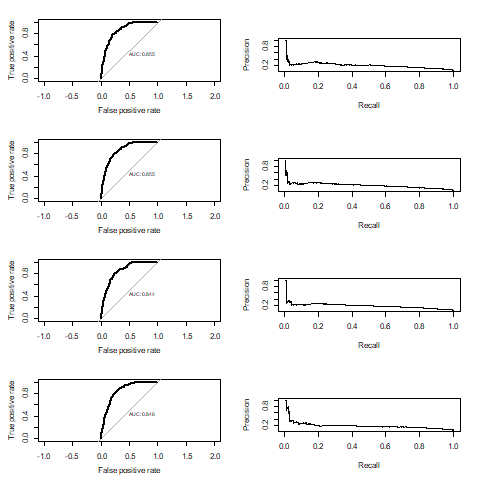
\includegraphics{curves.png}
\caption{roc and prec-rec curves, with the order: reduced model, interaction model, LDA model, QDA model.}
\end{figure}

Once fitting the models, we would like to see their performance in the
training set in order to have a first evaluation, hence for each
prediction we apply the associated threshold returned by the built-in
function.

\begin{Shaded}
\begin{Highlighting}[]
\NormalTok{mod.red.train.pred.class }\OtherTok{\textless{}{-}} \FunctionTok{as.numeric}\NormalTok{(mod.red.train.pred }\SpecialCharTok{\textgreater{}=}\NormalTok{ roc\_thresholds[}\DecValTok{1}\NormalTok{])}
\FunctionTok{table}\NormalTok{(training.set}\SpecialCharTok{$}\NormalTok{stroke,mod.red.train.pred.class, }\AttributeTok{dnn=}\FunctionTok{c}\NormalTok{(}\StringTok{\textquotesingle{}Ground thruth\textquotesingle{}}\NormalTok{,}\StringTok{\textquotesingle{}Reduced model }
\StringTok{            predicted\textquotesingle{}}\NormalTok{))}
\end{Highlighting}
\end{Shaded}
\newpage
\begin{verbatim}
##              Reduced model roc
##             predicted
## Ground thruth    0    1
##             0 2323 1199
##             1   13  147
\end{verbatim}

\begin{Shaded}
\begin{Highlighting}[]
\NormalTok{mod.red.train.pred.class }\OtherTok{\textless{}{-}} \FunctionTok{as.numeric}\NormalTok{(mod.red.train.pred }\SpecialCharTok{\textgreater{}=}\NormalTok{ recall\_thresholds[}\DecValTok{1}\NormalTok{])}
\FunctionTok{table}\NormalTok{(training.set}\SpecialCharTok{$}\NormalTok{stroke, mod.red.train.pred.class, }\AttributeTok{dnn=}\FunctionTok{c}\NormalTok{(}\StringTok{\textquotesingle{}Ground thruth\textquotesingle{}}\NormalTok{,}\StringTok{\textquotesingle{}Reduced model}
\StringTok{            predicted\textquotesingle{}}\NormalTok{))}
\end{Highlighting}
\end{Shaded}

\begin{verbatim}
##              Reduced model recall
##             predicted
## Ground thruth    0    1
##             0 1423 2099
##             1    1  159
\end{verbatim}

\begin{Shaded}
\begin{Highlighting}[]
\NormalTok{mod1.train.pred.class }\OtherTok{\textless{}{-}} \FunctionTok{as.numeric}\NormalTok{(mod1.train.pred }\SpecialCharTok{\textgreater{}=}\NormalTok{ roc\_thresholds[}\DecValTok{2}\NormalTok{])}
\FunctionTok{table}\NormalTok{(training.set}\SpecialCharTok{$}\NormalTok{stroke, mod1.train.pred.class, }\AttributeTok{dnn=}\FunctionTok{c}\NormalTok{(}\StringTok{\textquotesingle{}Ground thruth\textquotesingle{}}\NormalTok{,}\StringTok{\textquotesingle{}Interaction model }
\StringTok{            predicted\textquotesingle{}}\NormalTok{))}
\end{Highlighting}
\end{Shaded}

\begin{verbatim}
##              Interaction model roc
##             predicted
## Ground thruth    0    1
##             0 2314 1208
##             1   13  147
\end{verbatim}

\begin{Shaded}
\begin{Highlighting}[]
\NormalTok{mod1.train.pred.class }\OtherTok{\textless{}{-}} \FunctionTok{as.numeric}\NormalTok{(mod1.train.pred }\SpecialCharTok{\textgreater{}=}\NormalTok{ recall\_thresholds[}\DecValTok{2}\NormalTok{])}
\FunctionTok{table}\NormalTok{(training.set}\SpecialCharTok{$}\NormalTok{stroke, mod1.train.pred.class, }\AttributeTok{dnn=}\FunctionTok{c}\NormalTok{(}\StringTok{\textquotesingle{}Ground thruth\textquotesingle{}}\NormalTok{,}\StringTok{\textquotesingle{}Interaction model}
\StringTok{            predicted\textquotesingle{}}\NormalTok{))}
\end{Highlighting}
\end{Shaded}

\begin{verbatim}
##              Interaction model recall
##             predicted
## Ground thruth    0    1
##             0 1427 2095
##             1    1  159
\end{verbatim}

\begin{Shaded}
\begin{Highlighting}[]
\NormalTok{lda.fit.train.pred.class }\OtherTok{\textless{}{-}} \FunctionTok{as.numeric}\NormalTok{(lda.fit.train.pred}\SpecialCharTok{\textgreater{}=}\NormalTok{recall\_thresholds[}\DecValTok{3}\NormalTok{])}
\FunctionTok{table}\NormalTok{(training.set}\SpecialCharTok{$}\NormalTok{stroke, lda.fit.train.pred.class, }\AttributeTok{dnn=}\FunctionTok{c}\NormalTok{(}\StringTok{\textquotesingle{}Ground thruth\textquotesingle{}}\NormalTok{,}\StringTok{\textquotesingle{}LDA model}
\StringTok{            predicted\textquotesingle{}}\NormalTok{))}
\end{Highlighting}
\end{Shaded}

\begin{verbatim}
##              LDA model recall
##             predicted
## Ground thruth    0    1
##             0 1424 2098
##             1    1  159
\end{verbatim}

\begin{Shaded}
\begin{Highlighting}[]
\NormalTok{qda.fit.train.pred.class }\OtherTok{\textless{}{-}} \FunctionTok{as.numeric}\NormalTok{(qda.fit.train.pred}\SpecialCharTok{\textgreater{}=}\NormalTok{ recall\_thresholds[}\DecValTok{4}\NormalTok{])}
\FunctionTok{table}\NormalTok{(training.set}\SpecialCharTok{$}\NormalTok{stroke, qda.fit.train.pred.class, }\AttributeTok{dnn=}\FunctionTok{c}\NormalTok{(}\StringTok{\textquotesingle{}Ground thruth\textquotesingle{}}\NormalTok{,}\StringTok{\textquotesingle{}QDA model}
\StringTok{            predicted\textquotesingle{}}\NormalTok{))}
\end{Highlighting}
\end{Shaded}

\begin{verbatim}
##              QDA model recall
##             predicted
## Ground thruth    0    1
##             0 1759 1763
##             1    3  157
\end{verbatim}

From the confusion matrices of the first two examples of models we can
see a clear difference and effectiveness of the two designed
thresholds.\\
The ROC threshold tries to minimize the false positive errors by
considering just the positive results, instead the other one, as we see
from the output matrix, takes in consideration also the false negative
cases. Therefore it results to minimize more the false negative rate, by
allowing more errors for false positive values as counter-effect.

For our dataset by using the latter approach we have to highlight that
the number of FP has increased a lot, which still could be a major
problem, hence a good rates among these two metrics could be retrieved
depending on our desired result.\\
But as previously mentioned, in clinical cases an error committed to
diagnose a disease can be very dangerous, for example when instead of
predicting a stroke we classify it as a harmless case. For this reason,
from now onward, we will consider only the Recall-Precision optimal
threshold since it takes in consideration the False negative cases.

From the above confusion matrices we can already see which model is giving
the best result by looking at the FP and FN values of each fitting, in
particular we define the optimum choice which minimizes more both values
but by giving more importance to false negative minimization.

\hypertarget{model-validation}{%
\subsubsection{4.3.1 Model validation}\label{model-validation}}

A final assessment has to be done by seeing the performance of our
elective models on a set of data where they have not been trained on.
For this reason we will use the validation set that we defined
previously. In this manner we are able to simulate a real scenario case,
detect some possible overfitting issues, and by comparing the
performance of each model on this set we can finalize our choice.


In this phase the evaluation is again made by applying a threshold on
the predictions, in particular we will use the Precision-Recall
thresholds that we calculated in the training phase and see if the given
results are compliant to what we obtained on the training set. Moreover,
we will calculate the positive and negative error rates, which represent
the misclassification error on the prediction of having, or not, a
stroke.

\begin{Shaded}
\begin{Highlighting}[]
\CommentTok{\# Logistic reduced model}
\NormalTok{mod.red.val }\OtherTok{\textless{}{-}} \FunctionTok{predict}\NormalTok{(mod.red.train, val.set, }\AttributeTok{type=}\StringTok{"response"}\NormalTok{)}
\NormalTok{mod.red.val.class }\OtherTok{\textless{}{-}} \FunctionTok{as.numeric}\NormalTok{(mod.red.val }\SpecialCharTok{\textgreater{}=}\NormalTok{ recall\_thresholds[}\DecValTok{1}\NormalTok{])}
\NormalTok{conf.matr }\OtherTok{\textless{}{-}} \FunctionTok{table}\NormalTok{(val.set}\SpecialCharTok{$}\NormalTok{stroke, mod.red.val.class,  }\AttributeTok{dnn=}\FunctionTok{c}\NormalTok{(}\StringTok{\textquotesingle{}Ground thruth\textquotesingle{}}\NormalTok{,}\StringTok{\textquotesingle{}reduced model }
\StringTok{            predicted\textquotesingle{}}\NormalTok{))}
\FunctionTok{print}\NormalTok{(conf.matr)}
\end{Highlighting}
\end{Shaded}

\begin{verbatim}
##              reduced model 
##             predicted
## Ground thruth   0   1
##             0 497 681
##             1   1  48
\end{verbatim}

\begin{verbatim}
## [1] "Positive error rate is : 0.065844"
\end{verbatim}

\begin{verbatim}
## [1] "Negative error rate is : 0.002008"
\end{verbatim}

\begin{Shaded}
\begin{Highlighting}[]
\CommentTok{\# Logistic interaction model}
\NormalTok{mod1.val }\OtherTok{\textless{}{-}} \FunctionTok{predict}\NormalTok{(mod1.train, val.set, }\AttributeTok{type=}\StringTok{"response"}\NormalTok{)}
\NormalTok{mod1.val.class }\OtherTok{\textless{}{-}} \FunctionTok{as.numeric}\NormalTok{(mod1.val }\SpecialCharTok{\textgreater{}=}\NormalTok{ recall\_thresholds[}\DecValTok{2}\NormalTok{])}
\NormalTok{conf.matr }\OtherTok{\textless{}{-}} \FunctionTok{table}\NormalTok{(val.set}\SpecialCharTok{$}\NormalTok{stroke, mod1.val.class,  }\AttributeTok{dnn=}\FunctionTok{c}\NormalTok{(}\StringTok{\textquotesingle{}Ground thruth\textquotesingle{}}\NormalTok{,}\StringTok{\textquotesingle{}interaction model }
\StringTok{            predicted\textquotesingle{}}\NormalTok{))}
\FunctionTok{print}\NormalTok{(conf.matr)}
\end{Highlighting}
\end{Shaded}

\begin{verbatim}
##              interaction model 
##             predicted
## Ground thruth   0   1
##             0 499 679
##             1   1  48
\end{verbatim}

\begin{verbatim}
## [1] "Positive error rate is : 0.066025"
\end{verbatim}

\begin{verbatim}
## [1] "Negative error rate is : 0.002000"
\end{verbatim}

\begin{Shaded}
\begin{Highlighting}[]
\CommentTok{\# LDA model}
\NormalTok{lda.val }\OtherTok{\textless{}{-}} \FunctionTok{predict}\NormalTok{(lda.fit.train, val.set)}
\NormalTok{lda.val }\OtherTok{\textless{}{-}}\NormalTok{ lda.val}\SpecialCharTok{$}\NormalTok{posterior[, }\DecValTok{2}\NormalTok{]}
\NormalTok{lda.val.class }\OtherTok{=} \FunctionTok{as.numeric}\NormalTok{(lda.val }\SpecialCharTok{\textgreater{}=}\NormalTok{ recall\_thresholds[}\DecValTok{3}\NormalTok{])}
\NormalTok{conf.matr }\OtherTok{\textless{}{-}} \FunctionTok{table}\NormalTok{(val.set}\SpecialCharTok{$}\NormalTok{stroke, lda.val.class,  }\AttributeTok{dnn=}\FunctionTok{c}\NormalTok{(}\StringTok{\textquotesingle{}Ground thruth\textquotesingle{}}\NormalTok{,}\StringTok{\textquotesingle{}LDA model}
\StringTok{            predicted\textquotesingle{}}\NormalTok{))}
\FunctionTok{print}\NormalTok{(conf.matr)}
\end{Highlighting}
\end{Shaded}

\begin{verbatim}
##              LDA model
##             predicted
## Ground thruth   0   1
##             0 490 688
##             1   1  48
\end{verbatim}

\begin{verbatim}
## [1] "Positive error rate is : 0.065217"
\end{verbatim}

\begin{verbatim}
## [1] "Negative error rate is : 0.002037"
\end{verbatim}

\begin{Shaded}
\begin{Highlighting}[]
\CommentTok{\# QDA model}
\NormalTok{qda.val }\OtherTok{\textless{}{-}} \FunctionTok{predict}\NormalTok{(qda.fit.train, val.set)}
\NormalTok{qda.val }\OtherTok{\textless{}{-}}\NormalTok{ qda.val}\SpecialCharTok{$}\NormalTok{posterior[, }\DecValTok{2}\NormalTok{]}
\NormalTok{qda.val.class }\OtherTok{\textless{}{-}} \FunctionTok{as.numeric}\NormalTok{(qda.val }\SpecialCharTok{\textgreater{}=}\NormalTok{ recall\_thresholds[}\DecValTok{4}\NormalTok{])}
\NormalTok{conf.matr }\OtherTok{\textless{}{-}} \FunctionTok{table}\NormalTok{(val.set}\SpecialCharTok{$}\NormalTok{stroke, qda.val.class,  }\AttributeTok{dnn=}\FunctionTok{c}\NormalTok{(}\StringTok{\textquotesingle{}Ground thruth\textquotesingle{}}\NormalTok{,}\StringTok{\textquotesingle{}QDA model}
\StringTok{            predicted\textquotesingle{}}\NormalTok{))}
\FunctionTok{print}\NormalTok{(conf.matr)}
\end{Highlighting}
\end{Shaded}

\begin{verbatim}
##              QDA model
##             predicted
## Ground thruth   0   1
##             0 599 579
##             1   4  45
\end{verbatim}

\begin{verbatim}
## [1] "Positive error rate is : 0.072115"
\end{verbatim}

\begin{verbatim}
## [1] "Negative error rate is : 0.006633"
\end{verbatim}

As we did during the training phase, the evaluation is made by looking
at the false negative (FN) and false positive (FP) rates. The ratio of
the misclassified non-stroke people is almost zero in all models, so we
do not mistake for FN cases.

By running the code several times we saw that on average the reduced
model (\texttt{mod1}) slightly outperforms the other models, by
minimizing more the whole false rates, in addition we preferred it because it
allows us to give more insights of the predictors, as we saw in section
3.1.

\hypertarget{conclusions-and-further-analysis}{%
\section{5 Conclusions and Further
Analysis}\label{conclusions-and-further-analysis}}

As seen in the course of our analysis, we countered different problems.
In particular, many assumptions on the data and on the models have not
been satisfied by considering all the given predictors or by taking just
a subset of variables, for example the presence of collinearity, data
not Normal distributed, heteroscedasticity, high variance, and all the
other issues highlighted in the previous chapters.

The tests computed on our data involved various models, in which we have
included different combinations of predictors, even by mixing them
together to exploits and explore some synergy relationships.\\
Unfortunately the achieved complexity of the models is not enough for an
accurate stroke prediction. We still end up having a high amount of
false rates.\\
Furthermore, by looking at the plots generated in section 2.2
-Descriptive statistic- we can see that the data are not linearly
separable, thus it is not so easy to manage them by using linear models.

Despite the encountered predictiveness issues we still can highlight
many properties of the relationship among predictors and response
variables, in particular thanks to the explanatory analysis made on the
usage of logistic regression in this report.\\
For this reason after the training and validation phases, in which we
tested the models we have taken into account, we selected \texttt{mod1}
\[log\bigg(\frac{p(X)}{1-p(X)}\bigg) = \beta_0 + \beta_1\times \verb|age| + \beta_2\times \verb|avg_glucose_level| + \beta_3 \times \verb|heart_disease| \,+ \]
\[+\, \beta_4 \times\verb|hypertension| + \beta_5 \times \verb |age*heart_disease|\]
although it also guarantees slightly better performances than others.\\
In particular, in the \texttt{summary(mod1)} we can see how each feature
contributes on the prediction by looking at the \(\beta\) parameters.
The higher contribution on stroke comes from \texttt{heart\_disease}
with a coefficient equal to \(2.765\), even though its p-value is not
the smallest; the other features have all coefficient smaller than 1 but
are extremely important too, and highlight strong relationship with
having a stroke. Indeed, the strongest relation is always between
\texttt{stroke} and \texttt{age}, older people have a higher probability
to get a stroke and this disease will become an increasingly important
health problem as the world's population continues to age.

Furthermore, from this model we have been able to find some interactions
among \texttt{heart\_disease} and \texttt{age} as described in the
section 3.1.2, thanks to them we discovered that the response variable has
some effects by considering the people with heart disease and not.\\
Finally, we also saw that by considering the interaction we end up
having a high increment in the beta value of the heart disease variable.

Resuming the initial question, if it is possible to prevent a stroke, we
can answer that with our data we cannot achieve a secure prediction. Further analysis have to be explore considering other type of features
related with the stroke disease, in order to produce relevant results.\\
It has also to concern that more data should be collected especially for
people affected by stroke and also more correlated pathological variable
and health indicators should be considered too, by looking at the
available medical literature. These analysis and integration will allow
to build more reliable explanatory and predictive models.

\end{document}
